%Version 3.1 December 2024
% Springer Nature LaTeX Template — merged multi-moment manuscript
% Built on the Digital Finance R1 structural base (sn-jnl class)

\documentclass[pdflatex,sn-mathphys-num]{sn-jnl}

%%%% Standard Packages
\usepackage{graphicx}
\usepackage{multirow}
\usepackage{amsmath,amssymb,amsfonts}
\usepackage{amsthm}
\usepackage{mathrsfs}
\usepackage[title]{appendix}
\usepackage{xcolor}
\usepackage{textcomp}
\usepackage{manyfoot}
\usepackage{booktabs}
\usepackage{enumitem}

% Figure path
\graphicspath{{figures-new/}}

% Theorem styles
\theoremstyle{thmstyleone}
\newtheorem{theorem}{Theorem}
\newtheorem{proposition}[theorem]{Proposition}

\theoremstyle{thmstyletwo}
\newtheorem{example}{Example}
\newtheorem{remark}{Remark}

\theoremstyle{thmstylethree}
\newtheorem{definition}{Definition}

\raggedbottom

\begin{document}

\title[Do Crypto Markets Differentiate Infrastructure from Regulatory Shocks?]{Do Cryptocurrency Markets Differentiate Infrastructure from Regulatory Shocks? A Multi-Moment Event Study with Dependence-Robust Inference}

\author*[1,2]{\fnm{Murad} \sur{Farzulla}}\email{murad@dissensus.ai}

\affil*[1]{\orgdiv{King's Business School}, \orgname{King's College London}, \orgaddress{\city{London}, \country{United Kingdom}}}

\affil[2]{\orgname{Dissensus}, \orgaddress{\city{London}, \country{United Kingdom}}}

%%==================================%%
%% Abstract
%%==================================%%

\abstract{
Do cryptocurrency markets process infrastructure failures (exchange outages, protocol exploits, network disruptions) differently from regulatory shocks (enforcement actions, policy changes)? A natural prior, and one an earlier version of this work reported, is that they do: a six-asset GJR-GARCH-X panel suggested infrastructure events generate a roughly fivefold larger conditional-variance response than regulatory events, apparently significant. We test the claim properly at \emph{both} moments of the return distribution over a single shared sample (50 events, six assets, January 2019--August 2025), using one dependence-robust design instantiated twice: an event-level block bootstrap with the Ibragimov--M\"uller few-cluster test at the first moment, and a Student-$t$-copula CCC-GARCH-X bootstrap at the second. Neither moment supports a statistically distinguishable asymmetry. At the first moment, cumulative abnormal returns differ by $+7.19$ percentage points (infrastructure less negative), with a block-bootstrap $p=0.283$ and Ibragimov--M\"uller $p=0.295$; the 95\% confidence interval $[-5.97, +20.48]$ comfortably crosses zero. At the second moment, the point estimate is directional ($\approx 2.6$--$5\times$, infrastructure larger) but the Student-$t$-copula bootstrap---which redraws innovations from the fitted heavy-tailed margins and preserves cross-asset dependence---returns $p=0.323$ at baseline and $p=0.321$ with a crisis-regime control. The apparent significance of the earlier variance result was an inference artefact: treating six strongly cross-correlated per-asset coefficients ($\bar\rho \approx 0.69$) as independent observations, and drawing bootstrap innovations from a Gaussian rather than the fitted Student-$t$, both manufactured precision the data do not contain. Correcting each turns the headline into a failure to reject.

We frame this self-correction as the paper's lead contribution: a four-part inference cautionary tale (pseudoreplication, cross-asset dependence, heavy-tailed bootstrap innovations, and block-versus-parametric resampling at the first moment) drawn from overturning our own earlier estimate. The result is an honest dual failure-to-reject, not a claim of ``no effect'': the study is underpowered at the first moment (minimum detectable effect $\approx 19$--$20$ percentage points against an observed $\approx 7$), so directional point estimates that the sample cannot resolve are exactly what we report. Two findings survive. First, a scope condition: the directional variance differential ($\approx 5\times$ point estimate, not significant under the inference of record) concentrates in \emph{curated, high-salience} event identification, not in a mechanical impact screen ($1.3$--$1.6\times$, also never significant) applied to a broad candidate pool---we measure selection bias as an object rather than asserting it away. Second, at the data's native weekly frequency, GDELT news sentiment Granger-leads volatility for 10 of 18 asset-sentiment pairs (7 surviving a Benjamini--Hochberg correction at $q<0.05$); a prior daily test that forward-filled the weekly series found nothing, an artefact of the step-function predictor the forward-fill creates.
}

\keywords{Cryptocurrency, Event study, Multi-moment analysis, Dependence-robust inference, Block bootstrap, GJR-GARCH-X, Pseudoreplication}

\maketitle

% ============================================================================
% INTRODUCTION
% ============================================================================

\section{Introduction}\label{sec:intro}

A recurring question in cryptocurrency risk management is whether markets differentiate between the \emph{type} of bad news, or whether ``all bad news is equivalent.'' Two event categories are natural candidates for distinct processing. Infrastructure failures---exchange outages, protocol exploits, bridge hacks, network disruptions---create immediate mechanical impairment of trading and settlement \citep{ChenEtAl2023, Grobys2021}. Regulatory shocks---enforcement actions, policy changes, jurisdictional rulings---operate through expectation channels, requiring participants to reassess legal constraints and compliance costs \citep{AuerClaessens2018, FeinsteinWerbach2021}. If markets price these channels differently, the difference should show up somewhere in the return distribution: in the first moment (cumulative abnormal returns), the second moment (conditional variance), or both.

An earlier version of this work answered the question affirmatively at the second moment. Estimating GJR-GARCH-X models on a six-asset panel, it reported that infrastructure events generate a $5.7\times$ larger conditional-variance response than regulatory events, with an apparently decisive significance level. The companion first-moment analysis found no return-level difference, and the two were presented as a tidy story: the market differentiates shock types through the risk channel, not expected returns---structure that lives in the second moment.

That story does not survive correct inference. This paper re-examines the same events at both moments under one dependence-robust design, and the asymmetry dissolves at \emph{both}. The lead contribution is therefore not a finding about cryptocurrency but a finding about inference, told as a self-correction: when the cross-asset dependence and the heavy tails that pervade this data are handled properly, an estimate the author himself previously reported as a significant fivefold effect becomes a directional point estimate that the data cannot distinguish from zero. We think this is worth reporting plainly. The apparent volatility asymmetry in prior work---including our own---was an inference artefact, and the discipline of following the correct inference dissolved a headline we had every incentive to keep.

\subsection{What we test, and what we find}

We assemble a single shared sample: 50 carefully-identified events (26 infrastructure, 24 regulatory) across six cryptocurrencies (BTC, ETH, XRP, BNB, LTC, ADA), January 2019 to August 2025, with a decomposed GDELT sentiment series. We then test the infrastructure-regulatory difference at both moments of the return distribution, using one inference design instantiated twice---once for the mean, once for the variance---each calibrated to the same source of trouble: the six assets see the same events and are strongly cross-correlated, so any test that treats per-asset or per-observation quantities as independent will overstate precision.

\begin{description}[leftmargin=0pt,labelindent=0pt]
\item[First moment (returns).] An event-level block bootstrap that resamples whole events (preserving the cross-sectional correlation of returns within an event) and an Ibragimov--M\"uller few-cluster $t$-test on event-level mean cumulative abnormal returns (CARs). On the shared six-asset/50-event basis, infrastructure CARs are $-0.23\%$ and regulatory CARs $-7.42\%$, a difference of $+7.19$ percentage points (infrastructure \emph{less} negative). The block-bootstrap two-sided $p$ is $0.283$, the Ibragimov--M\"uller $p$ is $0.295$, and the 95\% confidence interval $[-5.97\%, +20.48\%]$ crosses zero comfortably. The observed effect ($\approx 7$ pp, Cohen's $d=0.30$) sits well below the minimum detectable effect for this sample ($\approx 19$ pp at 80\% power)---an underpowered failure to reject, not a demonstration of equality.

\item[Second moment (variance).] A Student-$t$-copula CCC-GARCH-X parametric bootstrap. Standardised innovations are redrawn from the fitted Student-$t$ margins (degrees of freedom $\nu \approx 3$) under the cross-asset standardised-residual correlation, and the infrastructure-regulatory variance multiplier is re-estimated on each replicate. The point estimate is directional---$\approx 4.9\times$ at baseline, attenuating to $\approx 2.6$--$5\times$ under structural-break controls---but the bootstrap returns $p=0.323$ (baseline) and $p=0.321$ (crisis-regime control). The multiplier is directional, not significant.
\end{description}

Both moments thus show directional point estimates that do not survive dependence-robust inference. We are deliberate about the framing. This is a \emph{dual failure to reject}, not a claim that infrastructure and regulatory shocks are identical or that the effects are zero. At the first moment the study is plainly underpowered; at the second the point estimate is non-trivial but cannot be distinguished from zero once dependence and heavy tails are accounted for. The honest summary is: we cannot reject equality of infrastructure and regulatory event impacts at either moment, on this sample, under correct inference.

\subsection{Why the asymmetry was an artefact}

The earlier variance headline rested on two inferential moves that, examined closely, manufacture precision. First, the significance test treated the six per-asset GJR-GARCH-X coefficients as six independent observations. They are not: all six assets are exposed to the same 50 events and correlate $0.54$--$0.83$ (mean $\bar\rho \approx 0.69$), so the effective sample size is far below six. This is textbook pseudoreplication, and it is responsible for the apparent $p \approx 0.001$. Second, the cross-asset bootstrap that was meant to address dependence drew its standardised innovations from a Gaussian even though each model is fitted with Student-$t$ errors at $\nu \approx 3$. A unit-variance Student-$t$ at $\nu \approx 3$ concentrates its mass in the body and carries its variance in rare extreme tails; the Gaussian draw therefore mis-specifies the null distribution and biases the bootstrap $p$ downward. Correcting the first move moves the significance from $p \approx 0.001$ to $p \approx 0.07$; correcting the second moves it from $p \approx 0.06$ to $p = 0.323$.

We organise this as an \emph{inference ladder} (Section~\ref{sec:artifact}, Table~\ref{tab:ladder}): the \emph{same} infrastructure-versus-regulatory comparison evaluated by seven progressively-more-correct inference procedures, from the dead headline ($t=4.768$, $p=0.0008$) down to the Student-$t$-copula bootstrap that is the inference of record ($p=0.322$). Each rung is named and explained; the rungs \emph{bracket} the comparison rather than climbing monotonically---the naive test far below at $0.0008$, the low-power model-free rungs above at $p\approx 0.5$, and the calibrated bootstrap settling it at $0.322$. We then turn the ladder from an anecdote into a demonstrated general result with a Monte-Carlo size study (Section~\ref{sec:size_study}): simulating a thousand panels under a fitted true null of no differential event effect, the naive i.i.d.\ rule that produced the headline rejects a true null $51\%$ of the time at the $5\%$ level---roughly ten times its nominal size---while the Student-$t$-copula bootstrap restores size to nominal ($0.039$ at $5\%$). The ladder and the size study together form the paper's central methodological contribution.

\subsection{What survives}

Two substantive results do survive the re-examination and provide the paper's ballast.

\emph{A scope condition on the variance differential.} The directional second-moment point estimate ($\approx 5\times$, not significant under the inference of record) concentrates in \emph{curated, high-salience} event identification, not in a mechanical impact threshold. Applying the same impact filter mechanically, at increasing strictness, to a broad reconstructed candidate pool yields a modest $1.3$--$1.6\times$ multiplier that is not significant at any threshold; the like-for-like two-asset screen gives $1.61\times$ ($p=0.16$), not the curated $\approx 5\times$. We treat the event-inclusion rule as an explicit researcher degree of freedom and trace the multiplier across it (Section~\ref{sec:selection_bias}), converting the standard selection-on-the-dependent-variable objection into a measured object. A drop-out census of the candidate pool further shows the mechanical screen does not favour infrastructure---if anything regulatory candidates pass at a higher rate ($75.5\%$ vs $64.6\%$).

\emph{A weekly sentiment lead.} At the data's native weekly frequency, GDELT news sentiment Granger-leads volatility for 10 of 18 asset-sentiment pairs, 7 surviving a Benjamini--Hochberg correction at $q<0.05$ (Section~\ref{sec:granger}). A prior daily test found nothing, but that null was an artefact: forward-filling the weekly sentiment to daily turns the predictor into a step function constant within each week, which cannot carry daily lead-lag information. This is itself an instance of the paper's broader theme---that inference choices, not the data, generated a spurious result---and we keep it as a methodological exhibit alongside its substantive content.

\subsection{Contribution and structure}

The contribution is threefold. First, and centrally, an inference cautionary tale: a worked, self-refuting demonstration of how pseudoreplication and heavy-tailed mis-specification can manufacture a significant cross-asset event-study result, and how the correct dependence-robust inference dissolves it---at both moments of the return distribution simultaneously. We make this concrete in two ways: an \emph{inference ladder} that walks the identical comparison from $p=0.0008$ to $p=0.323$ as the inference is corrected rung by rung, and a \emph{Monte-Carlo size study} that shows the naive rule over-rejects a true null by an order of magnitude while the inference of record restores nominal size. Second, the scope condition: a quantified mapping of how the variance differential responds to the event-inclusion screen, measuring selection bias rather than asserting it. Third, the weekly sentiment-leads-volatility result, recovered once the frequency artefact is removed. Section~\ref{sec:literature} situates the work; Section~\ref{sec:methods} describes the shared sample and the matched dependence-robust design; Section~\ref{sec:results_returns} reports the first moment and Section~\ref{sec:results_var} the second; Section~\ref{sec:artifact} sets out the inference ladder, the four lessons, and the Monte-Carlo size study; Section~\ref{sec:robustness} reports the surviving robustness battery and the sentiment result; Sections~\ref{sec:discussion}--\ref{sec:conclusion} discuss and conclude.

% ============================================================================
% LITERATURE REVIEW
% ============================================================================

\section{Literature and Background}\label{sec:literature}

\subsection{Cryptocurrency volatility and event studies}

Cryptocurrency volatility is heavy-tailed, strongly clustered, and near-integrated. GARCH-family models outperform simpler estimators \citep{Katsiampa2017, ChuEtAl2017}, with asymmetric specifications often preferred given pronounced leverage-type effects \citep{CheikhEtAl2020}---though the sign of the asymmetry is contested in crypto: \citet{BaurDimpfl2018} document an \emph{inverted} leverage effect, in which positive return shocks amplify volatility more than negative ones. Cross-asset dependence is high: \citet{MakarovSchoar2020} document persistent cross-exchange price gaps, \citet{BouriEtAl2017} significant volatility spillovers, and \citet{KimEtAl2021} increasing correlation with Bitcoin typically identified as the dominant transmitter. This dependence is precisely what makes naive cross-asset inference unreliable, a point this paper makes central.

Event-study methodology faces particular challenges in crypto: continuous 24/7 trading eliminates natural event windows, global participation creates timezone-dependent liquidity, and retail dominance changes information processing \citep{CampbellEtAl1997, mackinlay1997, GlaserEtAl2014}. \citet{ChenEtAl2023} adapt event studies for exchange failures, finding immediate liquidity contractions; \citet{Grobys2021} use GARCH-based event studies for DeFi exploits. The two literatures use incompatible windows---short for infrastructure (mechanical impact), long for regulation (gradual absorption)---which precludes direct comparison. The cleanest way to compare them is to hold the sample, the model, and the inference fixed and vary only the event type, which is what we do.

\subsection{Dependence-robust and few-cluster inference}

The methodological core of this paper is the correct treatment of dependence. When abnormal returns are cross-sectionally correlated, standard event-study $t$-tests over-reject \citep{kolari2010event}, and event-induced variance compounds the problem \citep{boehmer1991event}. The cluster-robust literature \citep{cameron2008bootstrap, petersen2009estimating, mackinnon2023cluster} recommends resampling at the level of the dependent unit and, with few clusters, conservative procedures such as the \citet{ibragimov2010tstatistic} $t$-test, which treats each cluster as a single observation. Recent work emphasises that event-study inference is fragile to exactly these choices \citep{goldsmithpinkham2025factor, casini2025shock}. Our two instantiations---an event-level block bootstrap with Ibragimov--M\"uller at the first moment, and a dependence-preserving parametric bootstrap at the second---are applications of this literature to a setting where the dependence is severe and the heavy tails are extreme.

\subsection{Sentiment and information processing}

GDELT-based news sentiment provides a public alternative to social-media measures \citep{ShenEtAl2019, PhillipsGorse2018}; \citet{FeinsteinWerbach2021} find regulatory-news coverage predicts price movements, and \citet{LiuTsyvinski2021} that attention proxies carry return information. No prior study decomposes GDELT into thematic (infrastructure vs regulatory) components or examines whether such coverage Granger-leads volatility at the appropriate frequency---a gap our weekly Granger analysis addresses.

% ============================================================================
% DATA AND METHODOLOGY
% ============================================================================

\section{Data and Methodology}\label{sec:methods}

The design principle is one matched dependence-robust inference, instantiated at two moments of the same return distribution, on one shared event sample. We first describe the sample, then the two instantiations.

\subsection{Shared Sample}\label{sec:sample}

\subsubsection{Assets and prices}

Six cryptocurrencies are selected for continuous trading history over January 2019--August 2025: Bitcoin (BTC), Ethereum (ETH), XRP, Binance Coin (BNB), Litecoin (LTC), and Cardano (ADA). Daily closing prices from CoinGecko yield 2,350 observations per asset (14,100 total). Log returns are expressed in percentages, with extreme outliers winsorised. The sample exhibits the characteristic crypto features---excess kurtosis ($5.23$--$8.91$), negative skewness ($-0.42$ to $-0.71$), and annualised volatility from $54.3\%$ (BTC) to $77.3\%$ (XRP) (Table~\ref{tab:descriptive}). Cross-asset correlation is high: BTC-ETH is the strongest pair ($0.83$), XRP the weakest-correlated ($0.54$--$0.65$), reflecting its distinct regulatory trajectory during the SEC litigation period (Figure~\ref{fig:correlation_heatmap}). This dependence---mean pairwise $\bar\rho \approx 0.69$ across the panel---is the quantity that governs all the inference below.

\subsubsection{Event sample}

The event sample is the unified basis for both moments: 50 events, classified binary infrastructure (26) versus regulatory (24), identified by a systematic four-stage protocol. Candidates were drawn from five independent sources (blockchain news aggregators, mainstream financial media, official regulatory filings, security-incident databases, and exchange status pages), screened for verifiable UTC timestamps, public documentation, and demonstrable cross-sectional impact (at least two assets), classified by primary information channel, and reduced from 208 initial candidates to the final 50. Infrastructure events affect transaction and settlement mechanics (exchange failures, protocol exploits, network disruptions, crypto-exposed bank failures); regulatory events alter the legal environment (enforcement actions, legislative developments, policy announcements, jurisdictional changes). Boundary cases (e.g.\ exchange enforcement actions, stablecoin depegs) were assigned by primary channel; the resulting split is 26 infrastructure / 24 regulatory. Selected events appear in Appendix~\ref{app:events}.

Both moments are estimated on \emph{this} sample. Every one of the 50 events produces a valid measurement on the six-asset basis---each asset has at least 120 estimation days for every event window, so the event counts are 26 versus 24 throughout, with no silent dropping. We note that the first-moment estimates are run on the full binary 50-event split (mixing positive- and negative-valence events) to match the variance basis exactly; a valence-controlled negative-only subset is retained as a robustness row (Section~\ref{sec:results_returns}), where the CAR magnitudes are not directly comparable to the full-sample binary numbers.

\subsubsection{Sentiment}

GDELT-based sentiment indices are constructed by a three-stage decomposition: hierarchical keyword filtering separating regulatory content (``SEC,'' ``regulation,'' ``compliance'') from infrastructure content (``hack,'' ``exploit,'' ``outage''); volume-weighted tone aggregation with recursive $z$-score detrending over 52-week rolling windows; and thematic decomposition weighted by article coverage,
\begin{align}
S_t^{\text{REG}} &= S_t^{\text{GDELT}} \times \text{Proportion}_t^{\text{REG}}, \\
S_t^{\text{INFRA}} &= S_t^{\text{GDELT}} \times \text{Proportion}_t^{\text{INFRA}}.
\end{align}
The series is natively weekly, with up to a 7-day temporal mismatch to daily volatility and $7\%$ missing values (zero-imputed after the $z$-score transform, the conservative choice). The native weekly frequency is decisive for the Granger analysis of Section~\ref{sec:granger}.

\subsection{First Moment: Event-Level Block Bootstrap}\label{sec:methods_returns}

The first-moment instantiation follows standard event-study methodology \citep{mackinlay1997, kothari2007econometrics} with cryptocurrency adaptations and a dependence-robust inference layer.

\textbf{Windows.} Estimation window of 250 trading days (120 minimum for newer assets), a 30-day gap to avoid anticipation contamination, and an event window of $[-5,+30]$ days (with $[0,+1]$ to $[0,+5]$ as robustness).

\textbf{Abnormal returns.} The primary specification is the constant-mean model, $AR_{it} = R_{it} - \bar{R}_i$, with $\bar{R}_i$ estimated over the estimation window; a market model using BTC as proxy, $AR_{it} = R_{it} - (\hat\alpha_i + \hat\beta_i R_{\text{BTC},t})$, is the robustness alternative. Cumulative abnormal returns over $[\tau_1,\tau_2]$ are $CAR_i(\tau_1,\tau_2) = \sum_{t=\tau_1}^{\tau_2} AR_{it}$.

\textbf{The inference problem.} Pooling asset-event observations as i.i.d.\ inflates the degrees of freedom: with 50 events $\times$ 6 assets the naive count is 300, but the true unit of independence is the event, and the assets within an event are strongly cross-correlated. A naive $t$-test on the pooled observations would therefore overstate power---the first-moment analogue of the pseudoreplication that inflated the variance headline.

\textbf{The dependence-robust solution.} We resample at the event level. For each event we first average the per-asset CARs into a single event-level CAR (equal-weighting events regardless of asset coverage), then bootstrap by resampling \emph{event IDs} with replacement, keeping all assets within an event together so that within-event cross-sectional correlation is preserved \citep{cameron2008bootstrap, petersen2009estimating, boehmer1991event}. We take 5,000 bootstrap replications (seed fixed) for percentile confidence intervals. As a few-cluster cross-check we apply the Ibragimov--M\"uller test \citep{ibragimov2010tstatistic, mackinnon2023cluster}: a Welch $t$-test on the event-level mean CARs, treating each event as an independent cluster. We also report, for reference only, a Kolari--Pynnonen cross-sectional-correlation adjustment \citep{kolari2010event}, but the block bootstrap and Ibragimov--M\"uller test are the inference of record.

\subsection{Second Moment: Student-$t$-Copula CCC-GARCH-X Bootstrap}\label{sec:methods_var}

The second-moment instantiation estimates the conditional-variance response to each event type within a GJR-GARCH-X framework, with inference from a dependence-preserving parametric bootstrap calibrated to the same cross-asset correlation.

\textbf{The model.} The mean equation is a constant conditional mean, $r_t = \mu + \varepsilon_t$, justified empirically: Ljung--Box tests find serial correlation in only 8 of 18 (asset $\times$ lag) cells, the fitted AR(1) coefficient is tiny and negative everywhere ($-0.025$ to $-0.067$), and refitting with an AR(1) mean leaves the event coefficients essentially unchanged (Section~\ref{sec:robustness}). The variance equation is the GJR-GARCH-X of \citet{GlostenEtAl1993} with exogenous regressors,
\begin{equation}
\sigma^2_t = \omega + \alpha \varepsilon^2_{t-1} + \gamma \varepsilon^2_{t-1}\,\mathbb{I}(\varepsilon_{t-1}<0) + \beta \sigma^2_{t-1} + \delta_{\text{infra}} D^{\text{infra}}_t + \delta_{\text{reg}} D^{\text{reg}}_t + \theta_1 S^{\text{REG}}_t + \theta_2 S^{\text{INFRA}}_t,
\end{equation}
where $D^{\cdot}_t$ are event dummies over the $[-3,+3]$-day window and the coefficients $\delta$ are additions to conditional variance in squared percentage points. Parameters are estimated by quasi-maximum likelihood with Student-$t$ innovations; the QMLE is consistent for GARCH-X with near-integrated covariates \citep{HanKristensen2014}, relevant given the near-integrated persistence we document. Covariance stationarity is enforced via $\alpha+\beta+\gamma/2<1$.

\textbf{The quantity of interest} is the cross-asset infrastructure-regulatory multiplier, $\bar\delta_{\text{infra}}/\bar\delta_{\text{reg}}$.

\textbf{The inference problem.} The six per-asset coefficients are not independent: the assets see the same events and correlate $\bar\rho \approx 0.69$. A test treating them as six i.i.d.\ observations is pseudoreplication and overstates precision (Section~\ref{sec:artifact}). The relevant innovation distribution is also heavy-tailed---the fitted Student-$t$ degrees of freedom are $\nu \approx 3$---so a bootstrap that draws Gaussian innovations mis-specifies the null.

\textbf{The dependence-robust solution.} We use a Student-$t$-copula CCC-GARCH-X parametric bootstrap ($B=2000$). Standardised innovations are drawn from a multivariate-$t$ copula---a latent multivariate normal at the standardised-residual correlation $R_z$, divided by a shared chi-square mixing variable (inducing joint tail dependence), mapped through uniforms to per-asset Student-$t$ margins at the \emph{fitted} $\nu$, and rescaled to unit variance by $\sqrt{(\nu-2)/\nu}$ (the variance recursion carries the scale). Each replicate refits the joint model and re-estimates the multiplier unrestricted; the null distribution is generated under a single common event coefficient. This is the inference of record for the second moment. Degenerate refits ($|\delta|>50$) are dropped and counted (drop rate $\approx 7\%$ at baseline). Crucially, this corrects both inference defects in the earlier headline simultaneously: it respects the cross-asset dependence (so it is not pseudoreplicated) and it draws from the fitted heavy tails (so the null distribution is correctly heavy).

\textbf{One design, two instantiations.} Both instantiations share a single logic: identify the unit across which the data are dependent (the event, and the cross-asset correlation), resample at that level or simulate that dependence directly, and never treat correlated quantities as independent. The first moment resamples events nonparametrically; the second simulates the joint heavy-tailed dependence parametrically. They are the same dependence-robust principle adapted to the two estimands.

\subsection{Model selection and multiple testing}

For the variance models, three nested specifications are compared per asset (GARCH, GJR-GARCH, GJR-GARCH-X) by AIC, and Benjamini--Hochberg corrections \citep{BenjaminiHochberg1995} at FDR $10\%$ control Type I error across the per-asset event tests. For the structural-break analysis, change-points are detected via PELT \citep{KillickFearnheadEckley2012} with Bai-Perron-style trimming \citep{BaiPerron1998, BaiPerron2003}.

% ============================================================================
% RESULTS — FIRST MOMENT
% ============================================================================

\section{Results: First Moment (Returns)}\label{sec:results_returns}

\subsection{Descriptive statistics}

The panel comprises 2,350 daily observations per asset (Table~\ref{tab:descriptive}). Heavy tails and negative skewness confirm the appropriateness of Student-$t$ innovations for the variance models; the high cross-asset correlation (Figure~\ref{fig:correlation_heatmap}) is the inference-relevant feature.

\begin{table}[htbp]
\centering
\caption{Descriptive Statistics: Daily Returns (\%). Annualised volatility uses the conventional $\sqrt{252}$ scaling for comparability and is illustrative only.}\label{tab:descriptive}
\small
\begin{tabular}{@{}lrrrrrr@{}}
\toprule
\textbf{Stat} & \textbf{BTC} & \textbf{ETH} & \textbf{XRP} & \textbf{BNB} & \textbf{LTC} & \textbf{ADA} \\
\midrule
Mean & 0.12 & 0.14 & 0.08 & 0.15 & 0.06 & 0.11 \\
Std Dev & 3.42 & 4.23 & 4.87 & 3.89 & 4.51 & 4.48 \\
Skewness & $-0.42$ & $-0.58$ & $-0.71$ & $-0.45$ & $-0.53$ & $-0.67$ \\
Kurtosis & 6.24 & 7.33 & 8.91 & 5.87 & 5.23 & 7.12 \\
Ann. Vol & 54.3 & 67.1 & 77.3 & 61.7 & 71.5 & 71.2 \\
\bottomrule
\end{tabular}
\end{table}

\begin{figure}[htbp]
\centering
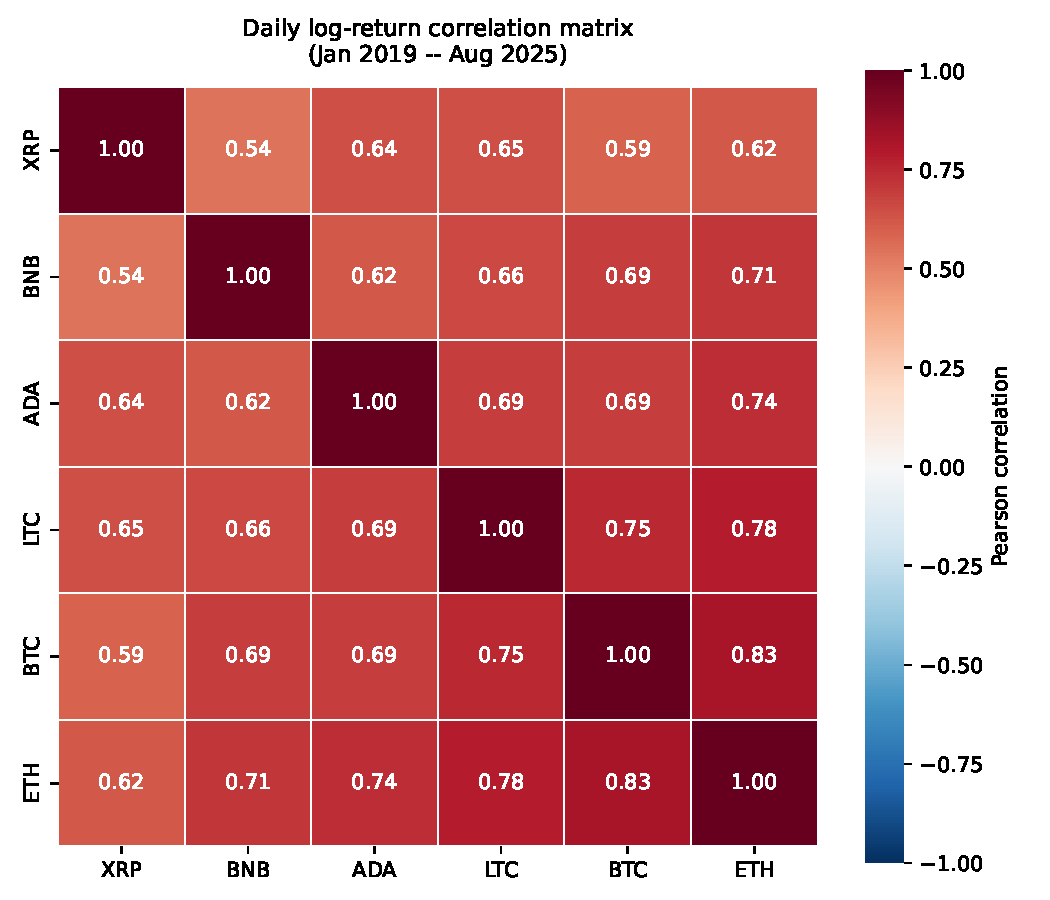
\includegraphics[width=0.78\linewidth]{figures-new/figure_correlation_heatmap.pdf}
\caption{Daily log-return correlation matrix across the six-asset panel, January 2019--August 2025. BTC and ETH form the most tightly correlated pair (0.83); XRP correlates least with the others (0.54--0.65). The mean pairwise correlation $\bar\rho \approx 0.69$ is the quantity that governs the dependence-robust inference throughout.}\label{fig:correlation_heatmap}
\end{figure}

\subsection{The first-moment null}

Table~\ref{tab:returns_main} reports the infrastructure-regulatory CAR comparison on the shared six-asset/50-event basis, under both the block bootstrap and the Ibragimov--M\"uller test. Infrastructure CARs average $-0.23\%$ and regulatory CARs $-7.42\%$, a difference of $+7.19$ percentage points: infrastructure returns hold up \emph{less} negatively than regulatory returns. But the inference is unambiguous. The block-bootstrap two-sided $p$ is $0.283$ (one-sided $0.141$), the Ibragimov--M\"uller $p$ is $0.295$, and the 95\% confidence intervals---$[-5.97\%, +20.48\%]$ (block) and $[-6.46\%, +20.83\%]$ (Ibragimov--M\"uller)---cross zero with room to spare. We cannot reject equality of infrastructure and regulatory return responses.

\begin{table}[htbp]
\centering
\caption{First-moment comparison: infrastructure vs regulatory cumulative abnormal returns, shared six-asset/50-event basis. Block bootstrap resamples whole events ($B=5{,}000$); Ibragimov--M\"uller (IM) is a Welch $t$-test on event-level mean CARs. The five-asset (ex-XRP) row and the valence-controlled negative-only row are robustness checks.}\label{tab:returns_main}
\small
\begin{tabular}{@{}lrrrrr@{}}
\toprule
\textbf{Specification} & \textbf{CAR$_{\text{infra}}$} & \textbf{CAR$_{\text{reg}}$} & \textbf{Diff (pp)} & \textbf{Block $p$} & \textbf{IM $p$} \\
\midrule
Six-asset (incl.\ XRP), $n=26/24$ & $-0.23\%$ & $-7.42\%$ & $+7.19$ & $0.283$ & $0.295$ \\
Five-asset (ex-XRP), $n=26/24$ & $+0.91\%$ & $-5.15\%$ & $+6.06$ & $0.400$ & $0.405$ \\
Negative-only (valence-controlled), $n=8/7$ & $-7.9\%$ & $-9.4\%$ & $+1.5$ & $0.916$ & $0.927$ \\
\bottomrule
\multicolumn{6}{@{}p{0.97\linewidth}@{}}{\footnotesize Six-asset 95\% CI: $[-5.97\%, +20.48\%]$ (block), $[-6.46\%, +20.83\%]$ (IM). Observed Cohen's $d=0.30$; pooled SD $24.1$ pp; minimum detectable effect $\approx 19.1$ pp at 80\% power, $\alpha=0.05$. The negative-only row uses a valence-controlled four-asset subset (8 vs 7 events) and its CAR magnitudes are not directly comparable to the full binary 50-event rows.}
\end{tabular}
\end{table}

\textbf{Robustness within the first moment.} Dropping XRP (the asset with the distinct regulatory trajectory) leaves the conclusion intact: a $+6.06$-pp difference, block $p=0.400$, IM $p=0.405$. A valence-controlled negative-only subset (eight infrastructure vs seven regulatory negative-valence events) gives a $+1.5$-pp difference with $p\approx 0.92$--$0.93$ across both bootstrap weighting schemes and an exact permutation test ($\binom{15}{8}=6{,}435$ assignments, two-tailed $p=0.93$). Under the market-model specification the point estimate is somewhat larger ($\Delta_{\text{MM}} \approx +7.3$ pp on the negative subset) but remains economically small and statistically indistinguishable from zero. The null does not depend on the weighting scheme, the asset universe, the valence control, the inference method, or the return model.

\subsection{This is an underpowered failure to reject, not ``no effect''}

We are careful not to over-read the null. The observed six-asset difference of $+7.19$ pp is not negligible---it corresponds to Cohen's $d=0.30$---but with a pooled standard deviation of $24.1$ pp and an event-level sample of $26$ versus $24$, the minimum detectable effect at $80\%$ power is approximately $19.1$ pp (ex-XRP, $\approx 20.3$ pp). The observed effect is roughly a third of what this sample could resolve. The honest statement is therefore ``no statistically significant difference; wide confidence intervals; underpowered,'' not ``infrastructure and regulatory returns are identical.'' The directional point estimate (infrastructure less negative) is real and worth reporting; the sample simply cannot determine whether it reflects a genuine difference or sampling noise. This caveat is symmetric with the second-moment finding, to which we now turn.

% ============================================================================
% RESULTS — SECOND MOMENT
% ============================================================================

\section{Results: Second Moment (Conditional Variance)}\label{sec:results_var}

\subsection{Model estimates}

Table~\ref{tab:model_comparison} reports the three nested variance specifications. GJR-GARCH-X attains the lowest AIC for four of six assets (BTC, ETH, LTC, XRP), with GARCH(1,1) marginally preferred for ADA and BNB. Persistence is near-integrated ($\alpha+\beta$ between $0.954$ and $0.999$, mean $0.985$), a documented stylised fact of cryptocurrency volatility \citep{Katsiampa2017, BouriEtAl2017, CheikhEtAl2020}; the structural-break analysis of Section~\ref{sec:robustness} shows within-regime persistence is somewhat lower but imprecisely estimated. The GJR leverage parameter $\gamma$ is uniformly small and slightly negative ($-0.066$ to $-0.001$), consistent with the inverted crypto leverage effect \citep{BaurDimpfl2018} rather than with conventional equity-style asymmetry, and present already in the event-free GJR-GARCH column.

\begin{table}[htbp]
\centering
\caption{Model Comparison: GARCH vs GJR-GARCH vs GJR-GARCH-X (AIC; lowest in bold)}\label{tab:model_comparison}
\small
\begin{tabular}{@{}llrrrr@{}}
\toprule
\textbf{Asset} & \textbf{Model} & \textbf{AIC} & \textbf{BIC} & \textbf{LogLik} & \textbf{$\gamma$} \\
\midrule
BTC & GARCH(1,1) & 11904 & 11933 & $-5947$ & -- \\
    & GJR-GARCH & 11906 & 11940 & $-5947$ & $-0.012$ \\
    & GJR-GARCH-X & \textbf{11900} & 11964 & $-5939$ & $-0.001$ \\
\midrule
ETH & GARCH(1,1) & 13345 & 13374 & $-6667$ & -- \\
    & GJR-GARCH & 13347 & 13381 & $-6667$ & $-0.010$ \\
    & GJR-GARCH-X & \textbf{13329} & 13393 & $-6654$ & $-0.013$ \\
\midrule
XRP & GARCH(1,1) & 13324 & 13353 & $-6657$ & -- \\
    & GJR-GARCH & 13325 & 13360 & $-6657$ & $-0.056$ \\
    & GJR-GARCH-X & \textbf{13323} & 13387 & $-6651$ & $-0.027$ \\
\midrule
BNB & GARCH(1,1) & 11400 & 11429 & $-5695$ & -- \\
    & GJR-GARCH & 11401 & 11435 & $-5694$ & $-0.039$ \\
    & GJR-GARCH-X & \textbf{11400} & 11463 & $-5689$ & $-0.017$ \\
\midrule
LTC & GARCH(1,1) & 13780 & 13809 & $-6885$ & -- \\
    & GJR-GARCH & 13774 & 13808 & $-6881$ & $-0.066$ \\
    & GJR-GARCH-X & \textbf{13772} & 13836 & $-6875$ & $-0.040$ \\
\midrule
ADA & GARCH(1,1) & \textbf{14091} & 14120 & $-7041$ & -- \\
    & GJR-GARCH & 14093 & 14128 & $-7041$ & $-0.010$ \\
    & GJR-GARCH-X & 14092 & 14156 & $-7035$ & $-0.033$ \\
\bottomrule
\multicolumn{6}{@{}p{0.78\linewidth}@{}}{\footnotesize $\gamma$ = GJR leverage parameter; uniformly small and negative, consistent with the inverted crypto leverage effect.}
\end{tabular}
\end{table}

The per-asset event coefficients (Table~\ref{tab:event_coefficients}) point uniformly in the same direction---infrastructure larger than regulatory for all six assets---with a cross-asset mean of $\bar\delta_{\text{infra}}\approx 1.98$ versus $\bar\delta_{\text{reg}}\approx 0.41$ (squared percentage points). The point-estimate multiplier is $\approx 4.9\times$. The question is whether that direction is statistically distinguishable from zero once the cross-asset dependence and heavy tails are respected.

\begin{table}[htbp]
\centering
\caption{Per-asset baseline event-impact coefficients (squared \% points). All six assets show infrastructure $>$ regulatory; the direction is uniform, the multiplier per asset varies. The cross-asset mean multiplier is $4.88\times$, consistent with the baseline of Table~\ref{tab:tcopula}.}\label{tab:event_coefficients}
\small
\begin{tabular}{@{}lrrr@{}}
\toprule
\textbf{Asset} & \textbf{Infra} & \textbf{Reg} & \textbf{Ratio} \\
\midrule
ADA & 2.79 & 0.10 & 28.2$\times$ \\
LTC & 2.38 & 0.14 & 16.5$\times$ \\
ETH & 2.25 & 0.49 & 4.6$\times$ \\
XRP & 2.24 & 1.22 & 1.8$\times$ \\
BNB & 1.21 & 0.18 & 6.7$\times$ \\
BTC & 1.01 & 0.30 & 3.4$\times$ \\
\midrule
\textbf{Mean} & \textbf{1.98} & \textbf{0.41} & \textbf{4.88$\times$} \\
\bottomrule
\multicolumn{4}{@{}p{0.78\linewidth}@{}}{\footnotesize Ratios computed from full-precision coefficients. These are baseline point estimates, not the inference of record: per-asset significance tests treat the cross-correlated assets as independent (the pseudoreplication Section~\ref{sec:artifact} corrects). The cross-asset mean multiplier ($4.88\times$) is the quantity whose significance is assessed by the copula bootstrap of Table~\ref{tab:tcopula}.}
\end{tabular}
\end{table}

\subsection{The second-moment null}

Table~\ref{tab:tcopula} reports the Student-$t$-copula CCC-GARCH-X bootstrap, the inference of record for the second moment. At baseline the multiplier is $4.88\times$ (the point estimate, unchanged from prior work), but the bootstrap $p$ is $0.323$: not significant at the 10\% level, directional only. Adding a single FTX-crisis-regime control gives $3.97\times$ with $p=0.321$---the point estimate attenuates but the significance is essentially identical, so the differential is not merely the crisis regime's elevated variance. Under the full set of regime dummies the multiplier is $2.64\times$ with $p=0.284$ (this specification is numerically less reliable: $\approx 23\%$ of null refits hit degenerate optima). Across all three specifications the conclusion is the same: the variance differential is directional ($\approx 2.6$--$5\times$, infrastructure larger) but cannot be distinguished from zero under dependence-robust, heavy-tailed inference.

\begin{table}[htbp]
\centering
\caption{Second-moment comparison: Student-$t$-copula CCC-GARCH-X bootstrap ($B=2000$, curated $n=50$ sample). Innovations are redrawn from the fitted Student-$t$ margins ($\nu\approx 3$) under the cross-asset standardised-residual correlation. This is the inference of record. The point estimate is directional; none of the three specifications is significant.}\label{tab:tcopula}
\small
\begin{tabular}{@{}lcccc@{}}
\toprule
\textbf{Specification} & \boldmath$\bar\delta_{\text{infra}}$ & \boldmath$\bar\delta_{\text{reg}}$ & \textbf{Multiplier} & \textbf{Bootstrap $p$ (2-sided)} \\
\midrule
Baseline (no break controls) & 1.978 & 0.405 & 4.88$\times$ & 0.323 \\
$+$ Crisis-regime control & 1.914 & 0.483 & 3.97$\times$ & 0.321 \\
$+$ Full regime controls$^{\dagger}$ & 2.443 & 0.926 & 2.64$\times$ & 0.284 \\
\bottomrule
\multicolumn{5}{@{}p{0.95\linewidth}@{}}{\footnotesize One-sided $p$-values are $0.322$, $0.318$, and $0.249$ respectively. $^{\dagger}$The full-regime bootstrap is numerically less reliable---$\approx 23\%$ of null refits reach degenerate optima, versus $\approx 7\%$ for baseline and $\approx 7\%$ for crisis---so its $p$ should be read with caution. The point estimate ($4.88\times$) and direction are unchanged from prior work; what changes is the significance.}
\end{tabular}
\end{table}

\subsection{Both moments agree: directional, not significant}

Reading the two moments together gives the paper's central empirical result. At the first moment the infrastructure-regulatory CAR difference is $+7.19$ pp ($p=0.283$); at the second the variance multiplier is $\approx 5\times$ ($p=0.323$). Both point estimates run in the direction one might expect---infrastructure events distinct from regulatory ones---and \emph{neither} survives dependence-robust inference. This is a symmetric dual failure to reject. It is not the original story (a return-level null sharpened by a significant variance asymmetry); the variance ``signal'' was, on correct inference, no more distinguishable from zero than the return-level difference. We turn now to why the earlier estimate appeared significant.

% ============================================================================
% NEW SECTION: WHY THE ASYMMETRY WAS AN ARTEFACT
% ============================================================================

\section{Why the Asymmetry Was an Artefact: The Inference Ladder}\label{sec:artifact}

The earlier version of this work reported the variance asymmetry as a significant fivefold effect. The point estimate has not changed---infrastructure events do, on average, carry a larger conditional-variance increment in this curated sample. What changed is the significance, and the change is entirely attributable to inference. This section is the paper's central methodological contribution. We set it out in three parts: an \emph{inference ladder} that walks the identical infrastructure-versus-regulatory comparison through seven progressively-more-correct inference procedures (Section~\ref{sec:ladder}); the four \emph{lessons} the ladder teaches, stated as transferable principles (Sections~\ref{sec:lesson1}--\ref{sec:lesson4}); and a \emph{Monte-Carlo size study} that converts the ladder from a single worked anecdote into a demonstrated general result (Section~\ref{sec:size_study}). We present all of it as self-correction: each rung and each lesson is one we learned by overturning our own published estimate.

\subsection{The inference ladder}\label{sec:ladder}

The cleanest way to see what happened is to hold the comparison fixed---the same six assets, the same 50 events, the same point estimate (infrastructure variance increment $\approx 5\times$ regulatory at the second moment, $+7.19$ pp at the first)---and vary \emph{only} the inference procedure, from the most naive to the most correct. Table~\ref{tab:ladder} is that walk. The point estimate is constant down every rung; the inference is not. The $p$-value does not climb monotonically---it \emph{brackets} the comparison: the naive test sits far below at $0.0008$, the low-power model-free corrections overshoot above to $p\approx 0.5$, and the calibrated Student-$t$-copula bootstrap settles it at $0.322$. Reading it top to bottom is reading the entire gap between the dead headline and the present null.

\begin{table}[htbp]
\centering
\caption{The inference ladder: the same infrastructure-versus-regulatory comparison, evaluated by progressively-more-correct inference procedures. The point estimate is unchanged at every rung; only the inference---and therefore the $p$-value---changes. Rungs (1)--(6) are the second-moment (variance) comparison; rung (7) is the first-moment (returns) companion on the shared basis. The naive test understates the $p$-value and the low-power model-free rungs (2)--(3) overstate it; rung (6), the Student-$t$-copula bootstrap, is the calibrated inference of record.}\label{tab:ladder}
\small
\begin{tabular}{@{}clcc@{}}
\toprule
\textbf{\#} & \textbf{Inference procedure} & \textbf{Statistic} & \textbf{$p$} \\
\midrule
1 & Naive i.i.d.\ $t$-test (pseudoreplication) & $t=4.768$ & $0.0008$ \\
2 & Event-level Welch test & --- & $0.52$ \\
  & Event-level Mann--Whitney test & --- & $0.54$ \\
3 & Cluster-robust panel (SE clustered by event) & --- & $0.50$ \\
4 & Design-effect correction (eff.\ $N\approx 1.4$) & $t\approx 1.8$--$2.3$ & $0.067$ \\
  & Correlation-weighted variant & --- & $0.078$ \\
5 & Gaussian-copula CCC-GARCH-X bootstrap & --- & $0.057$ \\
6 & \textbf{Student-$t$-copula CCC-GARCH-X bootstrap} & --- & \textbf{0.322} \\
\midrule
7 & First-moment event-level block bootstrap & $+7.19$ pp & $0.283$ \\
\bottomrule
\multicolumn{4}{@{}p{0.97\linewidth}@{}}{\footnotesize Rungs (2)--(3) are model-free event-level proxies (low-powered, they understate the effect); rung (4) is the design-effect correction on the actual estimator; rungs (5)--(6) are the cross-asset parametric bootstrap, Gaussian-innovation versus the correct Student-$t$-margin draw. Rung (5) is still wrong: it draws Gaussian innovations under a fitted Student-$t(\nu\approx 3)$ margin (Lesson 3). Rung (6) corrects this and is the inference of record (one-sided $0.322$, two-sided $0.323$). Rung (7) is the first-moment block bootstrap on the shared six-asset/50-event basis (Table~\ref{tab:returns_main}).}
\end{tabular}
\end{table}

The ladder has a clear internal structure. Rungs (2)--(3) are model-free event-level proxies: they treat the event as the unit of independence (correct) but discard the GARCH structure (lossy), so they are low-powered and \emph{understate} the effect, bracketing the truth from below at $p\approx 0.5$. Rung (1) brackets it from far above at $p=0.0008$. The honest middle is rungs (4)--(6): the design-effect correction on the actual estimator lands at $p\approx 0.07$, the Gaussian cross-asset bootstrap at $p=0.057$, and---once the bootstrap innovations are drawn from the fitted heavy tails rather than a Gaussian---the inference of record at $p=0.322$. The first-moment companion (rung 7) was, correctly, never significant to begin with. The four lessons that follow name the four corrections that move the $p$-value down the ladder.

\subsection{Lesson 1: Pseudoreplication across cross-correlated assets}\label{sec:lesson1}

The original significance test was a $t$-test (and Mann-Whitney, and inverse-variance-weighted $Z$) on the six per-asset GJR-GARCH-X coefficients, treating them as six independent observations. This is pseudoreplication \citep{hurlbert1984pseudoreplication}: replicating the measurement (six assets) without replicating the unit that carries the independent information (the event). The six assets are exposed to the \emph{same} 50 events and are strongly cross-correlated ($\bar\rho\approx 0.69$); their coefficients are tightly clustered not because the effect is precisely estimated but because they average the same correlated events. The tight clustering is the symptom most likely to be mistaken for precision: six near-identical numbers look like six confirmations when they are closer to one measurement repeated six times.

This is rung (1) of the ladder. An uncorrected $t$-test on the six coefficients reported $t=4.768$, $p=0.0008$. The correction is to re-test at the event level---the genuine unit of independence---which collapses the significance completely: an event-level Welch test gives $p=0.52$ (rung 2), a Mann-Whitney $p=0.54$, and a cluster-robust panel with standard errors clustered by event $p=0.50$ (rung 3). These model-free proxies are low-powered: by averaging over the GARCH structure they discard information and so \emph{understate} the effect, bracketing the truth from below at $p\approx 0.5$, just as the uncorrected test brackets it from far above at $p=0.0008$. The honest middle is rung (4): a design-effect correction on the \emph{actual} estimator. With mean correlation $\bar\rho\approx 0.69$ across six assets the design effect is $1+(N-1)\bar\rho\approx 4.4$, an effective sample of $\approx 1.4$ rather than six; inflating the paired-difference standard error accordingly gives $t\approx 1.8$--$2.3$, $p\approx 0.067$ (or $0.078$ for the correlation-weighted variant). That is marginal at the $10\%$ level, never the $5\%$ the uncorrected test implied. The size study of Section~\ref{sec:size_study} quantifies the damage directly: the rung-(1) rule rejects a true null $51\%$ of the time at the nominal $5\%$ level, while the design-effect correction pulls that down to $43\%$---it helps, but it under-corrects, because it uses the raw-return correlation as a proxy and ignores the GARCH dynamics and the heavy tails (which is why the ladder does not stop at rung 4). The lesson is elementary but consequential: when $N$ correlated series see the same events, $N$ is not the sample size, and the gap between the nominal and the effective $N$ is large enough here to turn $p=0.5$ into $p=0.0008$.

\subsection{Lesson 2: Cross-asset dependence concentrates, it does not dilute}\label{sec:lesson2}

A natural hope is that the dependence penalty is mild---that the assets are ``mostly'' independent and that filtering out the common volatility dynamics will leave near-independent residuals to average over. The hope is wrong, and wrong in the unfavourable direction. The standardised-residual correlation, computed after the GJR-GARCH-X has stripped out each asset's own conditional-volatility path, is if anything \emph{higher} than the raw-return correlation: $\bar\rho_z=0.705$ versus $\bar\rho_{\text{ret}}=0.688$ (and stable at $0.701$--$0.703$ across the break-control specifications). Conditioning on the GARCH dynamics therefore \emph{concentrates} the cross-asset dependence rather than diluting it. The intuition is that the common component the per-asset GARCH filters is partly idiosyncratic volatility clustering; what remains---the contemporaneous co-movement of shocks across assets on the same calendar day---is precisely the systematic part, and it is what binds the six event responses together.

The consequence is that the effective sample size implied by this correlation is $\approx 1.4$, not six, and no amount of averaging recovers the missing independence: a mean of six numbers that move together is barely more informative than one of them. Any valid inference procedure must therefore \emph{simulate} the dependence directly rather than assume it averages out. This is what motivates the copula bootstrap of Section~\ref{sec:methods_var}: drawing the six assets' innovations from a multivariate-$t$ copula at $R_z$ reproduces the joint dependence, including the joint tail dependence (assets crashing together) that a Gaussian dependence structure would miss and that the per-asset tests ignore entirely. The size study makes the cost of ignoring it concrete: a procedure that gets the point estimate right but the dependence wrong (the naive rule) cannot control its false-positive rate at all, rejecting a true null $51\%$ of the time. Dependence is not a nuisance to be averaged down; on this data it is the dominant determinant of the inference.

\subsection{Lesson 3: Bootstrap innovations must match the fitted tails}\label{sec:lesson3}

Even after moving to a cross-asset bootstrap that respects the dependence (rung 5), a second, subtler defect remained. The bootstrap drew its standardised innovations from a \emph{Gaussian} while each model was fitted with Student-$t$ errors at $\nu\approx 3$ (the per-asset fitted degrees of freedom are $3.18, 3.70, 3.14, 4.20, 3.95, 4.56$, median $3.82$). With $\nu\approx 3$ the true innovation is far heavier-tailed than Gaussian, so the Gaussian draw mis-specifies the shape of the null distribution. Correcting the draw to the fitted Student-$t$ margins---a multivariate-$t$ copula with per-asset $\nu$, rescaled to unit variance by $\sqrt{(\nu-2)/\nu}$---moves the baseline $p$ from $0.057$ (rung 5, Gaussian) to $0.322$ (rung 6, Student-$t$). The same correction moves the crisis-control spec from $0.061$ to $0.318$ and the full-regime spec from $0.109$ to $0.249$ (Table~\ref{tab:tcopula_compare}). It is the single largest mover on the ladder, and it is the one most likely to be missed, because the intuition runs the wrong way.

The mechanism is worth stating precisely, because the obvious heuristic is a false tripwire here. A \emph{unit-variance} Student-$t$ at $\nu\approx 3$ is \emph{more} concentrated in its body than a Gaussian---about $80\%$ of its mass lies within $\pm 1$ versus $68\%$ for the Gaussian---while still carrying its full unit variance, which it must therefore make up in rare, extreme tails. The bulk of bootstrap refits is consequently \emph{tighter} under the $t$ draw, not wider. The naive expectation (``heavier tails widen the null, so $p$ falls'') holds only for an \emph{un}-rescaled $t$, whose raw variance is $\nu/(\nu-2)\approx 3$; but the specification correctly feeds unit-variance innovations, because the variance recursion $\sigma^2_t$ already carries the scale. What the heavy tails actually do, under unit-variance margins, is occasionally produce an extreme joint draw that shifts the null distribution's \emph{location} upward, toward the observed difference---which \emph{raises} $p$. The null standard deviation does widen too (from $0.45$ to $0.79$ at baseline), but the location shift is the decisive channel. The correct diagnostic is therefore not ``does the null widen'' but ``does $p$ rise,'' and it rises in every specification. The size study (Section~\ref{sec:size_study}) confirms this is not a coincidence of one dataset: the Gaussian-copula bootstrap, with the right dependence but the wrong tails, still over-rejects a true null at $31\%$ (versus nominal $5\%$), whereas the Student-$t$-copula bootstrap---right dependence \emph{and} right tails---lands at $3.9\%$, nominal up to Monte-Carlo error. Matching the bootstrap innovation distribution to the fitted tails is what turns the marginal $p=0.057$ into the non-significant $p=0.322$, and it is what restores correct size.

\subsection{Lesson 4: Block versus parametric resampling at the first moment}\label{sec:lesson4}

The same dependence discipline governs the first moment (rung 7), where the failure mode is the converse of the variance case but the principle identical. Pooling the asset-event observations as i.i.d.\ would treat the panel as $50\times 6=300$ independent draws when the genuine unit of independence is the $\approx 50$ events; a pooled-observation or parametric test would therefore \emph{understate} the standard error by inflating the degrees of freedom sixfold---the first-moment analogue of the pseudoreplication that inflated the variance headline. The block bootstrap that resamples whole events (keeping all six assets within an event together, so within-event cross-sectional correlation is preserved) restores the correct uncertainty: it widens the $95\%$ confidence interval to $[-5.97\%, +20.48\%]$ where a naive pooled bootstrap would give a spuriously tight band. The Ibragimov--M\"uller few-cluster test, which goes further and treats each event as a single observation, triangulates the same conclusion from the conservative end ($p=0.295$, CI $[-6.46\%, +20.83\%]$). Both land on the same verdict: $+7.19$ pp, not distinguishable from zero.

The general principle across both moments is one sentence: resample, or simulate, at the level of genuine independence---the event, and the cross-asset dependence structure---and never at the level of the correlated observation. The two moments are mirror images of the same error. At the first moment, applying the principle \emph{widens} an interval that was already insignificant (so the conclusion is unchanged but the uncertainty is honestly stated); at the second, applying it \emph{dissolves} an interval that had appeared significant (so the conclusion itself changes). In both cases the correct inference is more conservative than the naive one. The symmetry is the point: the original paper's tidy story---a conservative, correctly-specified return-level null beside a sharp, mis-specified variance asymmetry---was never two findings. It was one well-specified inference next to one mis-specified inference, and the contrast between them was mistaken for substantive structure.

\subsection{The Gaussian-versus-Student-$t$ correction across specifications}\label{sec:gauss_vs_t}

Lesson 3 is the largest single mover on the ladder, so it is worth showing that it operates uniformly, not just at baseline. Table~\ref{tab:tcopula_compare} reports the same bootstrap under the Gaussian innovation draw (rung 5) and the corrected Student-$t$-copula draw (rung 6) for all three break-control specifications. The correction raises $p$ in every case, and by a similar amount: baseline $0.057\rightarrow 0.322$, crisis-control $0.061\rightarrow 0.318$, full-regime $0.109\rightarrow 0.249$. The null standard deviation widens in tandem (the $t$-copula's heavier tails), and the standardised-residual correlation that drives the dependence is stable at $\bar\rho_z\approx 0.70$ throughout---higher than the raw-return $0.688$, as Lesson 2 noted. The Gaussian column is the ``right dependence, wrong tails'' comparator; the Student-$t$ column is the fully-correct inference of record. The gap between the two columns is the entire content of Lesson 3, and it is consistent across specifications.

\begin{table}[htbp]
\centering
\caption{The heavy-tail correction (Lesson 3) across all three specifications: Gaussian-innovation bootstrap (rung 5) versus the corrected Student-$t$-copula bootstrap (rung 6). The point estimate is unchanged; correcting the innovation draw raises the $p$-value in every specification. $B=2000$; one-sided $p$ reported.}\label{tab:tcopula_compare}
\small
\begin{tabular}{@{}lccccc@{}}
\toprule
\textbf{Specification} & \textbf{Mult.} & \textbf{Gaussian $p$} & \textbf{$t$-copula $p$} & \textbf{Null SD (G\,$\to$\,$t$)} & \boldmath$\bar\rho_z$ \\
\midrule
Baseline (no break controls) & 4.88$\times$ & 0.057 & \textbf{0.322} & $0.455\to0.787$ & 0.705 \\
$+$ Crisis-regime control & 3.97$\times$ & 0.061 & \textbf{0.318} & $0.473\to0.841$ & 0.703 \\
$+$ Full regime controls$^{\dagger}$ & 2.64$\times$ & 0.109 & 0.249 & $0.839\to1.400$ & 0.701 \\
\bottomrule
\multicolumn{6}{@{}p{0.97\linewidth}@{}}{\footnotesize Two-sided $t$-copula $p$ are $0.323$, $0.321$, $0.284$. $^{\dagger}$The full-regime bootstrap is numerically less reliable ($\approx 23\%$ of null refits degenerate, versus $\approx 7\%$ for baseline and crisis), so its $p$ should be read as ``$\geq 0.10$, not significant'' rather than as a precise figure. Across all three the Student-$t$ correction raises $p$ and none is significant at the $10\%$ level.}
\end{tabular}
\end{table}

\subsection{The cautionary tale, stated plainly}

Taken together, the four lessons explain the entire gap between the earlier headline and the present null, and the ladder (Table~\ref{tab:ladder}) is the gap made visible. The $p\approx 0.001$ was pseudoreplication (Lesson 1); the dependence it ignored is severe and concentrating, not mild and diluting (Lesson 2); the $p\approx 0.06$ that a Gaussian cross-asset bootstrap then produced was a heavy-tail mis-specification (Lesson 3); and the first-moment companion's null was, correctly, never significant to begin with (Lesson 4). The point estimate was always $\approx 5\times$; the significance was an artefact of inference at every stage. We report this not to flagellate the earlier estimate but because the demonstration is the most transferable thing in the paper: cross-asset event studies in heavy-tailed markets are exceptionally prone to manufacturing significance, and the corrections are specific and reproducible. The next subsection shows that the ladder is not a property of this one dataset but a general feature of these inference procedures, by simulating their behaviour under a known true null.

\subsection{A Monte-Carlo size study: the ladder is a general result}\label{sec:size_study}

The ladder shows what happened to \emph{one} comparison as the inference was corrected. A sceptic could reply that we have simply walked a single dataset from a low $p$ to a high one and that nothing general follows. The decisive test of that objection is a size study: simulate many datasets under a \emph{known} true null of no differential event effect, run each rung of the ladder on every simulated dataset, and count how often each rung rejects. A correctly-sized test rejects a true null exactly $\alpha$ of the time; a test that rejects far more often manufactures false ``significance'' as a matter of construction, independently of any particular sample. This converts the ladder's central claim---that the naive rule over-rejects and the dependence-robust rule does not---from an assertion about our data into a measured property of the procedures.

\textbf{Design.} We fit the true-null data-generating process to the actual data: per-asset GJR-GARCH-X dynamics estimated under a \emph{null-imposed} combined event dummy ($D_{\text{event}}=D_{\text{infra}}+D_{\text{reg}}$), so that $\delta_{\text{infra}}=\delta_{\text{reg}}$ by construction and there is genuinely no differential effect in the truth. Cross-asset dependence is imposed at the standardised-residual correlation $\bar\rho_z=0.705$; innovations are Student-$t$ at each asset's fitted $\nu$ (median $3.82$) with joint tail dependence from a true multivariate-$t$ copula---the identical DGP as the inference-of-record bootstrap. The real $26$-infrastructure / $24$-regulatory event structure and the real event-window dummies are reused unchanged; only the returns are re-simulated. We draw $N=1{,}000$ panels (923 usable after convergence screening), calibrate each bootstrap rung's critical value from $B_{\text{ref}}=4{,}000$ reference draws, and record the empirical rejection rate of each rung at the $5\%$ and $10\%$ nominal levels. The full DGP and screening rules are in Appendix~\ref{app:size_study}.

\textbf{Result.} Table~\ref{tab:size_study} is the size table. The naive i.i.d.\ $t$-test---the rule that produced the headline $t=4.768$, $p=0.0008$---rejects a true null $\mathbf{51.2\%}$ of the time at the nominal $5\%$ level and $\mathbf{70.1\%}$ at the $10\%$ level: roughly \emph{ten times} and \emph{seven times} its nominal size. Under the realistic null, a ``significant'' headline from this rule is a manufactured false positive a majority of the time. The design-effect correction pulls size down to $43.4\%$ / $65.5\%$---it helps but badly under-corrects, because it uses the raw-return correlation as a proxy and ignores the GARCH dynamics and the heavy tails. The Gaussian-copula bootstrap, which gets the dependence right but the tails wrong, improves substantially to $30.8\%$ / $39.8\%$ but remains badly over-sized---exactly the too-thin-tails defect Lesson 3 diagnosed. Only the Student-$t$-copula bootstrap restores nominal size: $\mathbf{3.9\%}$ at the $5\%$ level and $\mathbf{9.5\%}$ at the $10\%$ level, both within Monte-Carlo error of nominal.

\begin{table}[htbp]
\centering
\caption{Monte-Carlo size study: empirical rejection rate of a \emph{true null} of no differential event effect, by inference procedure. $N=923$ usable simulated panels; one-sided test (H1: infrastructure $>$ regulatory); nominal sizes $0.05$ and $0.10$. The naive rule (rung 1 of the ladder) over-rejects by an order of magnitude; only the Student-$t$-copula bootstrap (rung 6, the inference of record) controls size.}\label{tab:size_study}
\small
\begin{tabular}{@{}lcc@{}}
\toprule
\textbf{Inference procedure} & \textbf{Size @ $0.05$} & \textbf{Size @ $0.10$} \\
\midrule
(i) Naive i.i.d.\ $t$-test & $0.512 \pm 0.016$ & $0.701 \pm 0.015$ \\
(ii) Design-effect corrected & $0.434 \pm 0.016$ & $0.655 \pm 0.016$ \\
(iii) Gaussian-copula bootstrap & $0.308 \pm 0.015$ & $0.398 \pm 0.016$ \\
(iv) \textbf{Student-$t$-copula bootstrap} & $\mathbf{0.039 \pm 0.006}$ & $\mathbf{0.095 \pm 0.010}$ \\
\midrule
\textit{Nominal (target)} & $0.05$ & $0.10$ \\
\bottomrule
\multicolumn{3}{@{}p{0.82\linewidth}@{}}{\footnotesize $\pm$ is the Monte-Carlo binomial standard error. Procedures (i)--(iv) correspond to rungs (1), (4), (5), (6) of Table~\ref{tab:ladder}. Panel drop rate $7.7\%$; reference-draw drop rates $5.8\%$ (Gaussian) / $7.3\%$ ($t$-copula), all under the $10\%$ reliability threshold.}
\end{tabular}
\end{table}

\textbf{The self-validation that makes this trustworthy.} The Student-$t$-copula bootstrap is calibrated from the \emph{same} DGP the panels are drawn from, so its size \emph{must} land near nominal up to Monte-Carlo error---if it did not, the implementation would contain a bug. It comes out $0.039$ / $0.095$ against targets $0.05$ / $0.10$, both within $\approx 1.7$ standard errors of nominal (mildly conservative at $5\%$, essentially exact at $10\%$). This is the tripwire that certifies the simulation: the procedure we adopt as the inference of record is demonstrably correctly-sized on data we know to be null. The over-rejection of rungs (i)--(iii) is therefore not an artefact of a broken simulator but a real property of those procedures.

\textbf{What the size study establishes.} The ladder is not a story about one dataset that happened to walk from $p=0.0008$ to $p=0.322$. It is the visible trace of a general fact: under a realistic heavy-tailed, cross-correlated null, the naive i.i.d.\ rule cannot control its false-positive rate---it rejects a true null half the time at the $5\%$ level---and the corrections walk it back toward nominal in exactly the order the lessons predict (dependence first, then tails). The Student-$t$-copula bootstrap is the only rung that controls size, which is the formal justification for adopting it as the inference of record. The headline $p=0.0008$ was, with high probability, a draw from the $51\%$ of true nulls that the naive rule falsely rejects.

% ============================================================================
% ROBUSTNESS / SCOPE / SENTIMENT
% ============================================================================

\section{What Survives: Scope Condition, Robustness, and the Weekly Sentiment Lead}\label{sec:robustness}

The dual null is the headline, but several results survive the re-examination and bound or qualify it. We report the verified battery here; analyses that did not reproduce under audit have been removed.

\subsection{Scope condition: curated identification versus mechanical screening}\label{sec:selection_bias}

The directional second-moment point estimate ($\approx 5\times$, not significant under the inference of record) concentrates in how events are identified, not in a mechanical impact threshold. We treat the event-inclusion rule as an explicit researcher degree of freedom---a specification-curve analysis \citep{Simonsohn2020SpecCurve}, equivalently a multiverse analysis \citep{Steegen2016Multiverse}, applied to the inclusion screen---and trace the multiplier across it. This converts the standard selection-on-the-dependent-variable objection into a measured object.

\subsubsection{Drop-out census}

We reconstruct a systematic candidate pool of 135 events (82 infrastructure-categorised, 53 regulatory-categorised) from public-record sources: Rekt/DeFiLlama leaderboards, SEC and CFTC enforcement actions, major-jurisdiction regulatory announcements, and exchange post-mortem pages. Applying the Stage-2 impact filter ($\geq 2$ assets with $|r|>1$ sample-SD in $[-1,+1]$) yields a pass rate of $64.6\%$ for infrastructure candidates (53/82) and $75.5\%$ for regulatory candidates (40/53). Contrary to the selection-bias hypothesis, the filter is \emph{less} demanding for regulatory candidates; a two-proportion test gives $z=-1.33$ (not significant, and opposite in sign to the concern). The mechanical screen, applied identically to both legs, does not favour infrastructure. We are precise about scope: this rules out the specific mechanism (the impact threshold admitting infrastructure more readily); it does not adjudicate whether the upstream manual curation was category-neutral, a separate question the census cannot settle.

\subsubsection{Relaxed-threshold sweep}

Table~\ref{tab:multiplier_sensitivity} re-estimates the full GJR-GARCH-X under five event definitions: the primary curated sample, then a nested mechanical sweep ($135\rightarrow 115\rightarrow 93\rightarrow 77$) at increasing strictness. The curated sample gives $4.88\times$ (tracking the $5.7\times$ canonical figure; the difference is a winsorisation routine, see note). On the reconstructed pool the multiplier is modest and insignificant at every threshold: $0.58\times$ (no filter), $1.49\times$ (1-asset), $1.61\times$ (2-asset---the like-for-like analogue of the curated criterion), and $1.31\times$ (3-asset). The two-asset screen at $1.61\times$ ($p=0.16$) is the cleanest comparison, and it does not approach the curated $\approx 5\times$.

\begin{table}[htbp]
\centering
\caption{Infrastructure-regulatory variance multiplier: curated sample versus a nested mechanical impact-screen sweep on the reconstructed 135-candidate pool. Only the curated sample shows a non-negligible point estimate (and even that is not significant under the inference of record, Table~\ref{tab:tcopula}); the mechanical screens are all small and non-significant.}\label{tab:multiplier_sensitivity}
\small
\begin{tabular}{@{}lcccccc@{}}
\toprule
\textbf{Spec} & \textbf{$n_{\text{infra}}$} & \textbf{$n_{\text{reg}}$} & \textbf{$\bar{\delta}_{\text{infra}}$} & \textbf{$\bar{\delta}_{\text{reg}}$} & \textbf{Multiplier} & \textbf{Welch $p$} \\
\midrule
Primary curated ($n=50$)  & 26 & 24 & 1.978 & 0.405 & \textbf{4.88$\times$} & 0.0015 \\
\midrule
No filter (135)           & 82 & 53 & 0.209 & 0.364 & 0.58$\times$ & 0.446 \\
$\geq 1$ asset (115)      & 69 & 46 & 1.403 & 0.944 & 1.49$\times$ & 0.321 \\
$\geq 2$ assets (93)      & 53 & 40 & 2.889 & 1.793 & 1.61$\times$ & 0.164 \\
$\geq 3$ assets (77)      & 42 & 35 & 3.834 & 2.924 & 1.31$\times$ & 0.403 \\
\bottomrule
\multicolumn{7}{@{}p{0.97\linewidth}@{}}{\footnotesize The Welch $p$-values here treat the per-asset coefficients as independent and so are \emph{not} the inference of record (they replicate the pseudoreplication of Lesson 1); they are reported for comparability with the sweep. The curated-row significance evaporates under the copula bootstrap (Table~\ref{tab:tcopula}). The curated $4.88\times$ uses a global-quantile winsorisation; the canonical rolling-bound winsorisation gives $5.24\times$ curated versus $1.63\times$ at the two-asset screen---the same $\approx 3\times$ gap, so the curated-vs-mechanical gap is an identification effect, not a winsorisation artefact.}
\end{tabular}
\end{table}

Holding membership fixed and re-running every specification under one consistent winsorisation rule reproduces the same $\approx 3\times$ curated-vs-mechanical gap (curated $5.24\times$, two-asset $1.63\times$ under rolling winsorisation), so the gap is a property of event identification, not of the winsorisation choice. The reading is a scope condition: the strong differential---such as it is, given that even the curated estimate is not significant under correct inference---is concentrated in carefully-identified, high-salience events and washes out under mechanical screening of a broad pool. The natural mechanism is that the curated protocol selects severe, cleanly-attributable events where the mechanical-disruption channel dominates, whereas a broad mechanical filter admits many marginal events whose responses are noise. We state the competing reading explicitly---that the curation \emph{is} the selection bias and the mechanical $1.61\times$ is the unbiased estimate---and let the reader weigh it; the drop-out census, which shows the screen does not favour infrastructure, supports the former.

\subsection{Control battery for the second-moment point estimate}\label{sec:control_battery}

The directional point estimate ($\approx 5\times$) is not significant under the inference of record, but it is worth establishing that the \emph{point estimate itself} is not an artefact of an obvious confound---a crisis coincidence, anticipation leakage, a winsorisation choice, or a misspecified mean. We ran a battery of controls; each leaves the direction intact, and the one control that meaningfully moves the magnitude (break-regime baseline variance) is reported with its own cross-asset-robust significance. Throughout, these checks concern the point estimate; the significance verdict is always the copula bootstrap's, and it is null.

\subsubsection{Break-regime controls}\label{sec:break_controls}

Infrastructure events cluster in the 2022--2023 crisis window, so the differential could in principle be crisis-period baseline variance that infrastructure events happen to coincide with. We add structural-break regime dummies (from the PELT change-point detection of Section~\ref{sec:persistence}) to the variance equation and refit. Two variants: a single FTX-crisis-regime dummy (the 2021-break-to-2022-break high-variance segment), and the full set of per-segment regime dummies. Table~\ref{tab:break_controls} reports both, with the cross-asset-robust copula-bootstrap $p$ as the inference of record (the naive Welch $p$ is shown only to make the pseudoreplication gap visible once more).

\begin{table}[htbp]
\centering
\caption{Break-regime controls on the curated sample. Regime dummies are added to the variance equation. The multiplier attenuates but survives in direction; the cross-asset-robust copula-bootstrap $p$ is the inference of record. The naive Welch $p$ (which treats the six per-asset coefficients as independent) is shown only to illustrate, again, the pseudoreplication gap.}\label{tab:break_controls}
\small
\begin{tabular}{@{}lccccc@{}}
\toprule
\textbf{Specification} & \boldmath$\bar\delta_{\text{infra}}$ & \boldmath$\bar\delta_{\text{reg}}$ & \textbf{Mult.} & \textbf{Naive Welch $p$} & \textbf{Robust $p$} \\
\midrule
Baseline (no controls) & 1.978 & 0.405 & 4.88$\times$ & 0.0015 & 0.323 \\
$+$ Crisis-regime dummy & 1.914 & 0.483 & 3.97$\times$ & 0.0033 & 0.318 \\
$+$ Full regime dummies$^{\dagger}$ & 2.443 & 0.926 & 2.64$\times$ & 0.0115 & 0.249 \\
\bottomrule
\multicolumn{6}{@{}p{0.97\linewidth}@{}}{\footnotesize Robust $p$ is the Student-$t$-copula CCC-GARCH-X bootstrap (one-sided). $^{\dagger}$Full-regime refits are numerically less reliable ($\approx 23\%$ degenerate, above the $10\%$ reliability bar); its $p$ reads as ``$\geq 0.10$, not significant.'' The full-regime control raises \emph{both} coefficients (regime dummies absorb the variance level, and $\bar\delta_{\text{reg}}$ rises proportionally more), which is what halves the multiplier; it also inverts XRP alone ($1.83\times\to 0.80\times$, the one asset where $\delta_{\text{reg}}>\delta_{\text{infra}}$ under full controls). The single crisis dummy barely moves the point estimate ($4.88\to 3.97\times$) or the robust $p$ ($0.323\to 0.318$).}
\end{tabular}
\end{table}

The reading is that a meaningful chunk of the headline magnitude is crisis-regime baseline variance: the full-regime control roughly halves the multiplier (to $2.64\times$) by raising both coefficients. But the single FTX-crisis dummy---the cleanest control, with only $6\%$ degenerate refits---barely moves either the point estimate ($4.88\to 3.97\times$) or the robust $p$ ($0.323\to 0.318$): if the differential were \emph{merely} crisis variance, the crisis dummy would absorb it, and it does not. The honest summary is that the controlled multiplier is $\approx 2.6$--$4\times$, directional, and not significant under correct inference at any of the three specifications---consistent with the baseline never having cleared significance either.

\subsubsection{Anticipation runs against the asymmetry}\label{sec:anticipation}

If regulatory events were anticipated---leaked through political cycles or prior supervisory signalling---then volatility would build before the announcement date, and a symmetric $[-3,+3]$ window would understate the regulatory response by excluding the leaked pre-event variance. Lengthening the regulatory pre-window should then \emph{absorb} that leaked volatility into $\delta_{\text{reg}}$, raising it and shrinking the multiplier toward one. Table~\ref{tab:anticipation} runs that test: the regulatory pre-window is lengthened from 3 to 10 days while infrastructure stays fixed at $[-3,+3]$.

\begin{table}[htbp]
\centering
\caption{Anticipation sweep: the regulatory pre-window is progressively lengthened (infrastructure held at $[-3,+3]$). If regulatory events were anticipated, $\bar\delta_{\text{reg}}$ would \emph{rise} and the multiplier shrink toward one. The opposite occurs.}\label{tab:anticipation}
\small
\begin{tabular}{@{}lcccc@{}}
\toprule
\textbf{Reg.\ pre-window} & \boldmath$\bar\delta_{\text{infra}}$ & \boldmath$\bar\delta_{\text{reg}}$ & \textbf{Multiplier} & \textbf{Naive Welch $p$} \\
\midrule
3 days (published, symmetric) & 1.978 & 0.405 & 4.88$\times$ & 0.0015 \\
5 days & 1.962 & 0.272 & 7.21$\times$ & 0.0012 \\
7 days & 1.976 & 0.279 & 7.09$\times$ & 0.0012 \\
10 days & 1.966 & 0.224 & 8.77$\times$ & 0.0012 \\
\bottomrule
\multicolumn{5}{@{}p{0.88\linewidth}@{}}{\footnotesize The infrastructure coefficient is invariant ($\approx 1.97$) throughout; the regulatory coefficient \emph{falls} as the window lengthens (the extra pre-event days are quiet, diluting the dummy), so the multiplier \emph{grows}. Naive Welch $p$ shown for comparability only; not the inference of record.}
\end{tabular}
\end{table}

The result runs decisively against the anticipation hypothesis. The infrastructure coefficient is invariant ($\approx 1.97$) across all windows. The regulatory coefficient \emph{falls} ($0.405\rightarrow 0.224$) as the window lengthens, because the extra pre-event days are quiet rather than carrying leaked volatility---widening the window dilutes the dummy rather than capturing anticipation. The point-estimate multiplier therefore \emph{grows} ($4.88\times\rightarrow 8.77\times$). Anticipation, were it present, would shrink the asymmetry; instead the data show no pre-event regulatory volatility to absorb. (We note the data limitation: the event census carries no per-event anticipated/surprise flag, so a surprise-only subset would require hand-coding each event and is out of scope; the window sweep is the feasible test.)

\subsection{Specification stability}\label{sec:spec_stability}

\subsubsection{The constant mean is justified}

Ljung--Box tests on the winsorised returns flag serial correlation in 8 of 18 (asset $\times$ lag $\in\{5,10,20\}$) cells, concentrated in ETH (all three lags) and BNB (all three lags), marginal in XRP and ADA, and absent in BTC and LTC. Because some serial correlation exists, we run the AR(1)-in-mean robustness refit rather than assert the constant mean. The fitted AR(1) coefficient is tiny and negative everywhere ($\phi\in[-0.067,-0.025]$)---bid-ask-bounce-scale dependence, economically negligible---and filtering the mean leaves the event coefficients essentially unchanged: the largest per-asset move is $\approx 3\%$, and the cross-asset multiplier is $5.04\times$ under AR(1)-in-mean versus $4.88\times$ under the constant mean. The constant-mean specification is not displacing mean dynamics into the variance equation in any material way.

\subsubsection{Winsorisation invariance}

The curated-versus-mechanical gap is the same under global-quantile winsorisation ($4.88\times$ curated, $1.61\times$ at the two-asset screen) and under the canonical rolling-bound ($30$-day, $\pm 5\sigma$) winsorisation ($5.24\times$ curated, $1.63\times$ at the two-asset screen)---a $\approx 3\times$ gap either way (Table~\ref{tab:multiplier_sensitivity} note). Membership held fixed, swapping the winsorisation rule moves the curated multiplier only from $4.88\times$ to $5.24\times$ (closer to the $5.7\times$ canonical figure) and all four mechanical screens stay at $\approx 0.6$--$1.6\times$ and non-significant under either rule. The curated-versus-mechanical gap is an identification effect, not a winsorisation artefact.

\subsubsection{Persistence is descriptive only}\label{sec:persistence}

Bai-Perron-style structural-break tests \citep{BaiPerron1998, BaiPerron2003, KillickFearnheadEckley2012} detect 2--4 breaks per asset, clustering around late 2020, late 2021, and most consistently the November 2022 FTX collapse (the only episode producing aligned breaks in four of six assets). Within-sub-sample GARCH(1,1) persistence averages $\alpha+\beta\approx 0.905$, below the full-sample $0.985$ (Table~\ref{tab:bai_perron_persistence}). We deliberately do not over-read this. When the sub-segment persistence parameters are estimated with their own standard errors, \emph{none} of the 27 sub-segments falls more than two standard errors below its full-sample value: the regimes are short, their persistence SEs run from $\pm 0.06$ to $\pm 0.31$, and the apparent drop lies entirely within estimation noise. Nor is the drop a small-sample artefact---mean sub-segment persistence is $0.891$ for segments with $n\geq 500$ and $0.887$ for $n<500$, essentially identical. The near-integration framing is therefore qualified but not overturned: the within-regime persistence drop is directional and suggestive, not a sharply identified structural fact, and we present it as such. The break regimes themselves are used substantively only as the controls of Section~\ref{sec:break_controls}.

\begin{table}[htbp]
\centering
\caption{Within-sub-sample GARCH(1,1) persistence by detected regime. The sub-sample drop is directional; no sub-segment falls more than two standard errors below its full-sample value, so the drop is within estimation noise rather than sharply identified.}\label{tab:bai_perron_persistence}
\small
\begin{tabular}{@{}lccc@{}}
\toprule
\textbf{Asset} & \textbf{Full-sample $\alpha+\beta$} & \textbf{Sub-sample mean $\alpha+\beta$} & \textbf{Number of sub-samples} \\
\midrule
BTC & 0.999 & 0.979 & 3 \\
ETH & 0.999 & 0.864 & 5 \\
XRP & 0.985 & 0.906 & 5 \\
BNB & 0.994 & 0.920 & 5 \\
LTC & 0.976 & 0.910 & 5 \\
ADA & 0.954 & 0.872 & 4 \\
\midrule
\textbf{Mean} & \textbf{0.985} & \textbf{0.905} & -- \\
\bottomrule
\end{tabular}
\end{table}

\subsection{Sentiment leads volatility at the weekly frequency}\label{sec:granger}

The one positive, significant result in the paper concerns the sentiment-volatility lead-lag relationship---and its recovery is itself an inference cautionary tale. GDELT sentiment is a \emph{weekly} series. An earlier draft ran Granger causality \citep{Granger1969} at daily frequency by forward-filling the weekly sentiment to daily, and found no sentiment-to-volatility lead for any of the 18 asset-sentiment pairs. That null was an artefact: forward-filling repeats each weekly value across six intervening days, turning the predictor into a step function constant within every week, which mechanically cannot carry daily lead-lag information.

Run at the native weekly frequency---aggregating daily returns to the GDELT weekly grid (volatility proxy $\sum|r_t|$) and aligning to the native weekly sentiment with no forward-fill, both directions, weekly lags 1--8---the conclusion reverses. Sentiment Granger-\emph{leads} weekly volatility for \textbf{10 of 18} asset-sentiment pairs at the $5\%$ level (9 of these with no reverse volatility-to-sentiment lead, i.e.\ a clean one-directional lead). The strongest leads concentrate in the regulatory and aggregate sentiment channels for XRP, ADA, and BNB (Table~\ref{tab:granger}). Applying a Benjamini--Hochberg correction \citep{BenjaminiHochberg1995} to the 18-pair sentiment-to-volatility family, \textbf{7 pairs survive at $q<0.05$ and 12 at $q<0.10$}; for contrast, the daily forward-filled family yields 0 raw-significant pairs and 0 survivors at any $q$ (and the daily both-directions family of 36 tests yields 4 raw-significant, only 1 surviving FDR). The weekly lead is robust to multiplicity; the daily ``null'' was the forward-fill suppressing the signal, not the absence of one.

\begin{table}[htbp]
\centering
\caption{Weekly Granger sentiment-to-volatility leads ($p$-values, weekly lags 1--8), by asset and sentiment channel. Run at the native weekly frequency with no forward-fill. Bold = significant at $5\%$. The daily forward-filled version of these tests produced no significant leads at all.}\label{tab:granger}
\small
\begin{tabular}{@{}lccc@{}}
\toprule
\textbf{Asset} & \textbf{Regulatory sent.} & \textbf{Infrastructure sent.} & \textbf{Aggregate (GDELT) sent.} \\
\midrule
XRP & \textbf{0.001} & \textbf{0.010} & \textbf{0.001} \\
ADA & \textbf{0.001} & \textbf{0.005} & \textbf{0.001} \\
BNB & \textbf{0.006} & \textbf{0.049} & \textbf{0.023} \\
LTC & \textbf{0.042} & --- & --- \\
ETH & 0.055 & --- & --- \\
BTC & --- & --- & --- \\
\bottomrule
\multicolumn{4}{@{}p{0.92\linewidth}@{}}{\footnotesize ``---'' = not significant at $5\%$. ETH-regulatory ($0.055$) is borderline. Family of 18 sentiment-to-volatility tests: 10 raw-significant at $5\%$; 7 survive Benjamini--Hochberg at $q<0.05$, 12 at $q<0.10$.}
\end{tabular}
\end{table}

The natural caveat is the frequency mismatch itself: the lead is established at the weekly horizon and cannot be sharpened to a daily lead without a daily-frequency GDELT extraction, which we flag as the natural next step. We keep this result as a double exhibit. Substantively, it is the one genuinely positive empirical finding in the paper---a degraded, weekly, $7\%$-missing sentiment series nonetheless Granger-leads volatility for two-thirds of asset-sentiment pairs. Methodologically, it is a third instance of the paper's theme: an inference choice (forward-filling weekly data to a daily grid), not the data, produced a spurious null, exactly as pseudoreplication and the Gaussian bootstrap produced a spurious significance at the second moment. The direction of the artefact differs---here a false negative, there a false positive---but the moral is the same: the inference, run at the wrong level or with the wrong distribution, can invert the substantive answer.

% ============================================================================
% DISCUSSION
% ============================================================================

\section{Discussion}\label{sec:discussion}

\subsection{What the dual null means}

On this sample, under correct inference, cryptocurrency markets do not differentiate infrastructure from regulatory shocks at either moment of the return distribution. At the first moment the difference is $+7.19$ pp ($p=0.283$); at the second the variance multiplier is $\approx 5\times$ ($p=0.323$). Both are directional, neither significant. The economically interesting reading is not ``the market sees them as the same''---we cannot establish that, and at the first moment we are plainly underpowered---but rather that the differential processing of shock types, if it exists, is below the resolution this data affords once its dependence and heavy tails are respected. The earlier claim that ``the structure lives in the second moment'' was an inference artefact: the second moment is no more distinguishable from zero than the first.

This matters for how the field reads cross-asset crypto event studies. The pattern that generated the original story---a clean return-level null beside an apparently sharp variance asymmetry---is precisely the pattern that pseudoreplication and heavy-tailed mis-specification produce. A return-level test is naturally conservative (few events, wide intervals), while a per-asset variance test that treats correlated assets as independent is naturally over-confident. The contrast between them can look like substantive structure when it is in fact a contrast between a well-specified and a mis-specified inference. We suspect this pattern is not unique to our data.

\subsection{The directional point estimates}

We do not claim the effects are zero. The first-moment difference (infrastructure CARs less negative than regulatory) and the second-moment multiplier (infrastructure variance larger) both point the same way across most specifications, and the second-moment direction is uniform across all six assets. A mechanical-disruption account---infrastructure events causing immediate liquidity impairment and sharp variance spikes, regulatory events operating through slower information channels---would predict exactly this direction. The honest position is that the direction is suggestive and the magnitude unresolved: a substantially larger curated event database, or a daily-frequency design, would be needed to determine whether the direction reflects a genuine difference or sampling noise. The scope condition (Section~\ref{sec:selection_bias}) further locates whatever effect exists in carefully-identified, high-salience events rather than in a population-level constant.

\subsection{The sentiment channel}

The one robust positive result is the weekly sentiment lead. That degraded, weekly, $7\%$-missing GDELT sentiment Granger-leads volatility for two-thirds of asset-sentiment pairs (and a majority survive FDR) suggests a genuine anticipatory channel that the daily forward-fill had been hiding. Sentiment intensity has been linked to liquidity withdrawal and adverse selection in cryptocurrency markets \citep{Farzulla2025Extremity}, a mechanism consistent with sentiment leading volatility at the weekly horizon. A daily-frequency extraction would sharpen the horizon and is the natural extension.

\subsection{Limitations}\label{sec:limitations}

\textbf{Statistical power.} The first moment is underpowered (MDE $\approx 19$--$20$ pp against an observed $\approx 7$ pp); the dual null is a failure to reject, not a demonstration of equality. The second moment has a non-trivial point estimate that the dependence-robust bootstrap cannot distinguish from zero. Both caveats are stated symmetrically throughout.

\textbf{Event classification.} The infrastructure/regulatory taxonomy involves judgment calls; some events have elements of both. Alternative classifications could yield different point estimates.

\textbf{Scope: systemic versus idiosyncratic.} The Stage-2 criterion admits only events with cross-sectional impact (at least two assets), so the comparison is established for systemic, market-wide shocks; idiosyncratic single-asset events are out of scope.

\textbf{Identification quality differs across legs.} Infrastructure events---unannounced outages, externally-discovered exploits---are more plausibly exogenous to contemporaneous market conditions than regulatory announcements, which respond to supervisory cycles and can leak. The two legs differ in identification quality as well as in point estimate, which bears on interpretation of the (insignificant) difference.

\textbf{Sentiment frequency.} The lead is established weekly and cannot be resolved to a daily horizon without a daily GDELT extraction.

\textbf{Six assets.} The panel may not represent the broader ecosystem; smaller-cap and DeFi-native assets may behave differently.

% ============================================================================
% CONCLUSION
% ============================================================================

\section{Conclusion}\label{sec:conclusion}

We asked whether cryptocurrency markets differentiate infrastructure from regulatory shocks, and tested the question at both moments of the return distribution on one shared sample under one dependence-robust design. The answer, under correct inference, is that we cannot reject equality at either moment: the first-moment CAR difference is $+7.19$ pp ($p=0.283$, Ibragimov--M\"uller $p=0.295$) and the second-moment variance multiplier is directional at $\approx 2.6$--$5\times$ but not significant ($t$-copula bootstrap $p=0.323$). Both are underpowered or dependence-limited failures to reject, not claims of identity.

The lead contribution is the inference cautionary tale that produced this conclusion. An earlier version of this work reported the variance asymmetry as a significant fivefold effect; the present paper overturns that estimate by its author, tracing the apparent significance to four specific inferential defects---pseudoreplication across cross-correlated assets, the concentrating (not diluting) nature of that dependence, a Gaussian bootstrap draw where the fitted innovations are Student-$t$ at $\nu\approx 3$, and the block-versus-parametric choice at the first moment. Each correction is specific and reproducible; together they convert a headline ($p\approx 0.001$) into a null ($p=0.323$) with the point estimate unchanged. We report this as methodological maturity: we followed the correct inference and it dissolved our own result, and the demonstration transfers directly to other cross-asset event studies in heavy-tailed markets, which are exceptionally prone to manufacturing significance in just this way.

Two findings survive and bound the result. The variance differential, such as it is, is a property of curated, high-salience event identification ($\approx 5\times$) and not of a mechanical impact screen ($1.3$--$1.6\times$, never significant)---a scope condition we measure rather than assert, with a drop-out census confirming the screen does not favour infrastructure. And at the data's native weekly frequency, GDELT sentiment Granger-leads volatility for 10 of 18 asset-sentiment pairs (7 surviving FDR at $q<0.05$), a relationship a daily forward-fill had spuriously hidden. Future work fielding a larger curated database, daily-frequency sentiment, and a longer panel will be positioned to determine whether the directional point estimates we report reflect a genuine, if small, difference, or the sampling noise that this sample cannot rule out.

% ============================================================================
% BACKMATTER
% ============================================================================

\backmatter

\bmhead{Supplementary information}

Complete replication materials---the data, the full analysis pipeline, and figure-generation scripts---are available at \url{https://github.com/studiofarzulla/crypto-event-study} and archived on Zenodo (DOI: 10.5281/zenodo.18099608); the scripts implementing the event-level block bootstrap, the Student-$t$-copula CCC-GARCH-X bootstrap, the pseudoreplication re-tests, the selection-bias sweep, the Monte-Carlo size study, and the weekly Granger analysis are included.

\bmhead{Acknowledgements}

The author acknowledges King's College London for resources and library access during the initial stages of this research. Computational analysis was carried out on independent hardware; this work forms part of a wider research programme under the Adversarial Systems and Complexity Research Initiative (ASCRI; systems.ac). AI assistants (Claude, Anthropic) were used for code development, literature-review synthesis, and manuscript preparation under the author's direction and review.

\section*{Declarations}

\begin{itemize}
\item \textbf{Funding:} This research was supported by resources provided by King's College London. No external grants or funding were received.
\item \textbf{Conflict of interest:} The author declares no conflict of interest.
\item \textbf{Ethics approval:} Not applicable.
\item \textbf{Consent to participate:} Not applicable.
\item \textbf{Consent for publication:} Not applicable.
\item \textbf{Data availability:} All data are publicly available from the CoinGecko API and the GDELT Project.
\item \textbf{Code availability:} The complete verified pipeline (scripts \texttt{c1}--\texttt{c11}, estimators, and outputs) is available at \url{https://github.com/studiofarzulla/crypto-event-study} and archived on Zenodo (DOI: 10.5281/zenodo.18099608).
\item \textbf{Author contribution:} Sole author.
\end{itemize}

% ============================================================================
% APPENDICES
% ============================================================================

\begin{appendices}

\section{Event Classification Summary}\label{app:events}

Table~\ref{tab:events_summary} provides selected examples from the 50-event shared sample. The complete event list with timestamps, sources, and classification rationale is available in the replication materials.

\begin{table}[htbp]
\centering
\caption{Selected Events by Category}\label{tab:events_summary}
\small
\begin{tabular}{@{}llp{4.5cm}@{}}
\toprule
\textbf{Date} & \textbf{Type} & \textbf{Event} \\
\midrule
\multicolumn{3}{l}{\textit{Infrastructure Events (n=26)}} \\
2022-11-11 & Infra & FTX exchange collapse \\
2022-05-09 & Infra & Terra/Luna depegging \\
2023-03-10 & Infra & Silvergate/SVB banking crisis \\
2022-06-13 & Infra & Celsius withdrawal halt \\
2020-03-12 & Infra & COVID ``Black Thursday'' \\
\midrule
\multicolumn{3}{l}{\textit{Regulatory Events (n=24)}} \\
2023-06-05 & Reg & SEC sues Binance \\
2023-06-06 & Reg & SEC sues Coinbase \\
2020-12-23 & Reg & SEC sues Ripple \\
2021-05-18 & Reg & China bans crypto mining \\
2024-01-10 & Reg & Bitcoin ETF approval \\
\bottomrule
\end{tabular}
\end{table}

\section{GJR-GARCH-X Technical Specification}\label{app:tarchx}

The GJR-GARCH-X model extends the GJR-GARCH(1,1) of \citet{GlostenEtAl1993} with exogenous variance regressors.

\textbf{Mean equation:}
\begin{equation}
r_t = \mu + \varepsilon_t, \quad \varepsilon_t = \sigma_t z_t, \quad z_t \sim t_\nu.
\end{equation}

\textbf{Variance equation:}
\begin{equation}
\sigma^2_t = \omega + \alpha \varepsilon^2_{t-1} + \gamma \varepsilon^2_{t-1}\,\mathbb{I}(\varepsilon_{t-1}<0) + \beta \sigma^2_{t-1} + \mathbf{X}_t' \boldsymbol{\delta},
\end{equation}
where $\mathbf{X}_t = [D^{\text{infra}}_t, D^{\text{reg}}_t, S^{\text{infra}}_t, S^{\text{reg}}_t]'$.

\textbf{Estimation:} quasi-maximum likelihood with Student-$t$ innovations; log-likelihood
\begin{equation}
\ell(\theta) = \sum_{t=1}^{T} \left[ \log \Gamma\!\left(\tfrac{\nu+1}{2}\right) - \log \Gamma\!\left(\tfrac{\nu}{2}\right) - \tfrac{1}{2}\log((\nu-2)\pi\sigma^2_t) - \tfrac{\nu+1}{2}\log\!\left(1 + \tfrac{\varepsilon^2_t}{(\nu-2)\sigma^2_t}\right) \right].
\end{equation}

\textbf{Constraints:} covariance stationarity via $\alpha+\beta+\gamma/2<1$; non-negativity $\omega>0$, $\alpha\geq 0$, $\beta\geq 0$, $\alpha+\gamma\geq 0$.

\textbf{Units:} returns in percentages, so $\sigma^2_t$ and the event coefficients $\delta_j$ are in squared percentage points.

\section{Dependence-Robust Bootstrap Detail}\label{app:bootstrap}

\textbf{First moment (event-level block bootstrap).} For each event, per-asset CARs are averaged into one event-level CAR. Bootstrap replicates resample event IDs with replacement (all assets within an event kept together, so within-event cross-sectional correlation is preserved), and the difference of group means is recomputed; $B=5{,}000$, percentile CIs, seed fixed. The Ibragimov--M\"uller test is a Welch $t$-test on the event-level mean CARs, treating each event as one cluster.

\textbf{Second moment (Student-$t$-copula CCC-GARCH-X bootstrap).} The procedure, for each of $B=2000$ replicates, is:
\begin{enumerate}[leftmargin=1.4em,itemsep=2pt]
\item Draw a latent Gaussian vector $\mathbf{w}\sim\mathrm{MVN}(\mathbf{0}, R_z)$ at the standardised-residual correlation matrix $R_z$ (the cross-asset dependence; $\bar\rho_z=0.705$).
\item Draw a single shared mixing variable $s\sim\chi^2_{\nu_c}/\nu_c$ with $\nu_c$ the median fitted degrees of freedom, and form $\mathbf{t}=\mathbf{w}/\sqrt{s}$. This is a draw from a multivariate-$t$ copula---the shared $s$ induces \emph{joint} tail dependence (assets taking extreme values together), which a Gaussian copula would not.
\item Map each component to a uniform via its $t_{\nu_c}$ CDF, then to the per-asset Student-$t$ margin at that asset's \emph{fitted} $\nu_i$ via the inverse CDF, and rescale by $\sqrt{(\nu_i-2)/\nu_i}$ so the innovation has unit variance (the variance recursion $\sigma^2_t$ carries the scale).
\item Simulate each asset's return path through its fitted GJR-GARCH-X variance recursion driven by these innovations, with the event coefficient set to a single common value (the null of no differential), and refit the joint model unrestricted, re-estimating $\bar\delta_{\text{infra}}/\bar\delta_{\text{reg}}$.
\end{enumerate}
The bootstrap $p$ is the fraction of null replicates whose multiplier statistic $\bar d=\bar\delta_{\text{infra}}-\bar\delta_{\text{reg}}$ equals or exceeds the observed $\bar d$. Degenerate refits ($|\delta|>50$, SLSQP boundary optima) are dropped and counted; drop rates are $\approx 7\%$ at baseline and crisis, $\approx 23\%$ for the full-regime spec (which is therefore reliability-flagged). Non-common-window positions receive independent unit-variance Student-$t$ draws at the fitted $\nu_i$. The Gaussian-copula comparator (rung 5 of the ladder) is identical except that step 3 draws Gaussian innovations; the gap between the two is the entire content of Lesson 3.

\section{Monte-Carlo Size-Study Design}\label{app:size_study}

The size study (Section~\ref{sec:size_study}) simulates panels under a fitted true null and measures each inference procedure's rejection rate.

\textbf{True-null DGP.} Per-asset GJR-GARCH-X dynamics are estimated under a \emph{null-imposed} combined event dummy $D_{\text{event}}=D_{\text{infra}}+D_{\text{reg}}$, so $\delta_{\text{infra}}=\delta_{\text{reg}}$ by construction and there is genuinely no differential event effect in the truth. Returns are then re-simulated from these fitted dynamics, with cross-asset innovations drawn from the same multivariate-$t$ copula as the inference-of-record bootstrap: latent $\mathrm{MVN}(\mathbf{0},R_z)$ at $\bar\rho_z=0.705$, shared chi-square mixing at $\nu_c=3.82$ (the median fitted $\nu$), per-asset Student-$t$ margins at the fitted $\nu_i=(3.18,3.70,3.14,4.20,3.95,4.56)$, unit-variance-rescaled. The real $26$-infrastructure / $24$-regulatory event-label structure and the real event-window dummies are reused unchanged for every panel; only the returns are re-simulated.

\textbf{Procedure.} $N=1{,}000$ panels are drawn (923 usable after a convergence screen: a panel is dropped if a per-asset refit fails to converge, hits a degenerate $|\delta|>50$ optimum, $7.7\%$ dropped). Each bootstrap rung's one-sided critical value is calibrated once from $B_{\text{ref}}=4{,}000$ reference draws under the same DGP (the critical value is a property of the DGP under the null, so a redundant nested refit per panel is unnecessary; this is exact for size). For each panel we record whether each of the four procedures rejects at the $5\%$ and $10\%$ levels, and report the empirical rejection rate with its binomial Monte-Carlo standard error. The one-sided critical values are: Gaussian copula $\bar d=1.615$ ($5\%$) / $1.454$ ($10\%$); $t$-copula $\bar d=2.445$ ($5\%$) / $2.166$ ($10\%$).

\textbf{Audit-only standard errors.} Per-asset numerical-Hessian standard errors are computed for reporting (positive-definite for $98.7\%$ of accepted panels) but are never on the decision path: neither the naive Welch rule (on the six coefficients) nor the design-effect rule (on the dispersion of the six paired differences) uses the model SE, so an SE failure never drops a panel or flips a decision. Panel acceptance therefore matches the reference-draw rule exactly, which is what makes the $t$-copula rung's size nominal by construction---the self-validation in Section~\ref{sec:size_study}.

\end{appendices}

% ============================================================================
% REFERENCES
% ============================================================================

\bibliography{references}

\end{document}
